\documentclass[11pt,a4paper]{article}
\usepackage[margin=2.25cm]{geometry}
\usepackage{fontspec}
\setmainfont{Arial}
\setsansfont{Arial}
\usepackage[spanish,es-nodecimaldot]{babel}
\usepackage{amsmath,amssymb}
\usepackage{graphicx}
\usepackage{booktabs,longtable,array,tabularx}
\usepackage{float}
\usepackage{xcolor}
\usepackage{hyperref}
\usepackage{fancyhdr}
\usepackage{enumitem}
\usepackage{listings}
\usepackage{caption}
\usepackage{microtype}

\definecolor{azul}{HTML}{174A6E}
\definecolor{gris}{HTML}{F1F4F6}
\definecolor{codigo}{HTML}{1F2933}
\hypersetup{colorlinks=true,linkcolor=azul,urlcolor=azul,citecolor=azul,pdftitle={Informe técnico del modelo DMI TerraBovina}}
\pagestyle{fancy}
\fancyhf{}
\lhead{Modelo DMI TerraBovina}
\rhead{Informe técnico}
\cfoot{\thepage}
\setlength{\headheight}{14pt}
\setlength{\parindent}{0pt}
\setlength{\parskip}{5pt}
\setlist{nosep,leftmargin=1.4em}
\captionsetup{font=small,labelfont=bf}
\lstset{basicstyle=\ttfamily\small,backgroundcolor=\color{gris},frame=single,rulecolor=\color{gray!35},breaklines=true,showstringspaces=false,columns=fullflexible,keywordstyle=\color{azul}\bfseries,stringstyle=\color{green!40!black},commentstyle=\color{gray}}
\newcommand{\archivo}[1]{\texttt{\detokenize{#1}}}
\newcommand{\DMI}{\textit{DMI}}

\begin{document}

{\LARGE\bfseries Informe técnico integral del modelo de estimación de consumo de materia seca TerraBovina}\par
\vspace{0.4em}
{\large Análisis del código, los datos, el proceso ETL, los modelos, las métricas, los gráficos y la inferencia}\par
\vspace{0.6em}
\textbf{Estado analizado:} repositorio local y artefactos disponibles al 23 de julio de 2026.\\
\textbf{Alcance:} documento académico universitario basado en el código y los resultados efectivamente presentes.

\tableofcontents
\newpage

\section{Resumen ejecutivo}

El proyecto desarrolla un sistema de aprendizaje automático para estimar el \textbf{consumo diario de materia seca} de un bovino, expresado como \archivo{dmi_kg_dia} en kilogramos de materia seca por animal y por día. El modelo recibe cuatro características: peso vivo, categoría animal, condición corporal y estado fisiológico normalizado. El problema se formula como una \textbf{regresión supervisada}: a partir de observaciones cuyo consumo ya se conoce, se aprende una función capaz de producir estimaciones para nuevos animales.

El conjunto disponible contiene \textbf{3.833 observaciones}, \textbf{17 columnas}, \textbf{1.639 identificadores animales} y \textbf{131 hogares o fincas} de Bomet, Kenia. La validación tiene en cuenta la estructura por hogar mediante cinco particiones de \archivo{StratifiedGroupKFold}: las observaciones de una misma finca no se reparten entre entrenamiento y prueba. Así se evita una forma importante de fuga de información y se mide la generalización hacia hogares no vistos dentro del mismo origen geográfico.

Se comparan cuatro alternativas: un baseline que predice la media, regresión Ridge, Random Forest y CatBoost. Ridge obtiene el menor MAE global: \textbf{1,1019 kg MS/día}, con RMSE de \textbf{1,5354} y $R^2$ de \textbf{0,6821}. CatBoost queda prácticamente empatado, con MAE de 1,1027; la diferencia es apenas 0,0008 kg MS/día. Por lo tanto, Ridge es el ganador según la regla implementada, pero no hay evidencia estadística suficiente para afirmar una superioridad robusta frente a CatBoost.

El resultado se serializa en \archivo{models/dmi_model.joblib}; las métricas y metadatos se escriben en \archivo{reports/model_metrics.json}; además se generan ocho gráficos de diagnóstico. Para inferencia, la clase \archivo{HerdPredictor} acepta lotes de animales, devuelve DMI absoluto y relativo al peso vivo, y advierte cuando un peso queda fuera del rango histórico de su categoría.

La conclusión debe interpretarse con prudencia: el sistema supera ampliamente al baseline y presenta un diseño metodológico razonable para evaluación interna, pero no dispone de un conjunto de prueba externo, del CSV crudo original ni de variables como clima, raza, composición de dieta, calidad del forraje o producción láctea. No corresponde usarlo directamente para decisiones nutricionales en Argentina sin validación local.

\section{Contexto, problema y objetivos}

\subsection{Materia seca y DMI}

La materia seca es la fracción del alimento que permanece una vez retirada el agua. Expresar el consumo en materia seca permite comparar alimentos con contenidos de humedad distintos. En este proyecto, DMI proviene de \textit{Dry Matter Intake} y representa la cantidad de materia seca consumida diariamente. La variable objetivo es cuantitativa continua, por lo que el problema no consiste en clasificar animales, sino en estimar un valor numérico.

Además del consumo absoluto, el sistema informa el consumo como porcentaje del peso vivo:
\begin{equation}
\text{DMI \% PV}=\frac{\text{DMI (kg/día)}}{\text{peso vivo (kg)}}\times100.
\end{equation}
Esta variable es útil para contextualizar el consumo entre animales de tamaños diferentes. Sin embargo, no se utiliza como entrada del modelo porque en el dataset se calcula a partir del propio objetivo; incluirla produciría \textbf{fuga de información}.

\subsection{Objetivo general}

Construir, evaluar y conservar un modelo reproducible que estime \archivo{dmi_kg_dia} a partir de variables disponibles por animal, comparando distintos enfoques de regresión y controlando la separación de hogares durante la validación.

\subsection{Objetivos específicos}
\begin{itemize}
  \item Validar, limpiar y normalizar los datos mediante un proceso ETL modular.
  \item Definir un contrato común de características para entrenamiento e inferencia.
  \item Comparar un punto de referencia, un modelo lineal regularizado y dos modelos de árboles.
  \item Medir el error con MAE, RMSE y $R^2$, globalmente, por fold y por categoría.
  \item Seleccionar el modelo de menor MAE fuera de muestra y reentrenarlo con todos los registros.
  \item Serializar el modelo junto con metadatos, limitaciones y rangos históricos.
  \item Proporcionar predicción por lotes y advertencias de extrapolación.
\end{itemize}

\section{Tecnologías y dependencias}

El proyecto está implementado en Python y se ejecuta como una colección de módulos y scripts locales. No contiene una API web, contenedores Docker, interfaz gráfica ni servicio desplegado.

\begin{longtable}{p{3.2cm}p{2.2cm}p{9cm}}
\toprule
\textbf{Tecnología} & \textbf{Versión declarada} & \textbf{Función en el proyecto}\\
\midrule
\endhead
Python & No fijada & Lenguaje principal. En el entorno revisado se encontró Python 3.13.14.\\
pandas & $\geq2.2,<4$ & Lectura y escritura de CSV, DataFrames, limpieza, selección y resumen de datos.\\
NumPy & No declarada & Arreglos de predicciones, valores nulos, truncamiento a cero y operaciones numéricas. Se importa directamente, pero no figura de forma explícita en \archivo{requirements.txt}.\\
scikit-learn & $\geq1.6,<2$ & Preprocesamiento, pipelines, validación cruzada, baseline, Ridge, Random Forest y métricas.\\
CatBoost & $\geq1.2.8,<2$ & Regresor de gradient boosting con variables categóricas declaradas.\\
Joblib & $\geq1.4,<2$ & Serialización y carga del bundle final.\\
Matplotlib & $\geq3.8,<4$ & Construcción y exportación de figuras.\\
Seaborn & $\geq0.13,<1$ & Estilo y gráficos estadísticos.\\
tqdm & $\geq4.67,<5$ & Barra de progreso de los 21 ajustes de entrenamiento.\\
pytest & $\geq8.3,<10$ & Framework previsto para pruebas automáticas; las pruebas no están presentes en el árbol actual.\\
JSON / pathlib & Biblioteca estándar & Metadatos, entrada/salida de prueba y gestión portable de rutas.\\
\bottomrule
\end{longtable}

Las restricciones son rangos y no versiones exactas; tampoco existe un lockfile. En consecuencia, una instalación futura puede resolver versiones diferentes y modificar resultados o compatibilidad. Para reproducibilidad estricta deberían registrarse Python, sistema operativo, \archivo{pip freeze}, hash del CSV, hash del modelo y commit de Git.

\section{Arquitectura y organización del repositorio}

La arquitectura separa datos, código, modelos y reportes:
\begin{lstlisting}
Modelo-IA-Py/
|-- data/processed/terrabovina_dmi_kenya_features V2.csv
|-- models/dmi_model.joblib
|-- reports/
|   |-- etl_summary.json
|   |-- model_metrics.json
|   `-- figures/ (8 archivos PNG)
|-- src/
|   |-- config.py
|   |-- etl/{extract.py, transform.py, load.py, run_etl.py}
|   |-- model/{features.py, train.py, predictor.py}
|   `-- visualization/plots.py
|-- testReal/{ejecutar.py, input.json, output.json}
|-- README.md
`-- requirements.txt
\end{lstlisting}

\subsection{Responsabilidad de los componentes}

\archivo{src/config.py} centraliza rutas con \archivo{pathlib.Path}. Esto evita distribuir cadenas de rutas por el código. \archivo{src/etl} implementa extracción, transformación y carga. \archivo{src/model/features.py} define el contrato de variables y una preparación común para entrenamiento e inferencia. \archivo{src/model/train.py} contiene la experimentación, selección y persistencia. \archivo{src/model/predictor.py} ofrece inferencia por lotes. \archivo{src/visualization/plots.py} genera los diagnósticos. \archivo{testReal} funciona como interfaz simple basada en JSON.

El flujo principal es:
\begin{center}
CSV fuente $\rightarrow$ extracción $\rightarrow$ transformación $\rightarrow$ CSV procesado $\rightarrow$ características $\rightarrow$ validación de modelos $\rightarrow$ Ridge final $\rightarrow$ Joblib/JSON/gráficos $\rightarrow$ predicción.
\end{center}

\section{Dataset y análisis descriptivo}

\subsection{Dimensión y unidad observacional}

El archivo \archivo{data/processed/terrabovina_dmi_kenya_features V2.csv} tiene 3.833 filas y 17 columnas. Contiene 1.639 identificadores animales y 131 hogares. Al existir múltiples mediciones por animal y cuatro periodos, los registros no deben interpretarse como 3.833 individuos independientes. Se trata de datos longitudinales o repetidos.

No se encontraron filas completamente duplicadas. Hay 2.194 filas cuyo identificador ya había aparecido antes, hecho compatible con mediciones repetidas. Los periodos contienen 783, 1.042, 1.016 y 992 observaciones respectivamente.

\subsection{Diccionario de datos}

\small
\begin{longtable}{p{3.5cm}p{1.7cm}r p{8cm}}
\toprule
\textbf{Columna} & \textbf{Tipo} & \textbf{Nulos} & \textbf{Interpretación y uso}\\
\midrule
\endhead
\archivo{animal_id} & texto & 0 & Identificador del animal o medición. Se devuelve en inferencia, pero no predice.\\
\archivo{hh} & entero & 0 & Hogar o finca. Se usa para agrupar la validación.\\
\archivo{kenya_category} & texto & 0 & Categoría original en inglés; no entra al modelo.\\
\archivo{categoria_terrabovina} & texto & 0 & Vaca, Vaquilla, Novillo, Toro o Ternero/Ternera. Entrada categórica.\\
\archivo{periodo} & entero & 0 & Periodo de observación; no entra al modelo.\\
\archivo{periodo_fechas} & texto & 0 & Intervalo textual; no entra al modelo.\\
\archivo{fecha_inicio} & texto & 291 & Fecha inicial; no entra al modelo.\\
\archivo{fecha_fin} & texto & 202 & Fecha final; no entra al modelo.\\
\archivo{peso_vivo_kg} & decimal & 0 & Peso vivo en kg. Principal entrada numérica.\\
\archivo{condicion_corporal} & decimal & 2.111 & Condición corporal. Se utiliza únicamente para vacas.\\
\archivo{dmi_kg_dia} & decimal & 0 & Objetivo: consumo diario de materia seca.\\
\archivo{dmi_pct_peso_vivo} & decimal & 0 & Variable derivada del objetivo; excluida para evitar fuga.\\
\archivo{outlier_peso} & booleano & 0 & Bandera de peso atípico; todos los valores actuales son falsos.\\
\archivo{outlier_dmi_abs} & booleano & 0 & Bandera de DMI absoluto atípico; todos falsos.\\
\archivo{outlier_dmi_pct_bw} & booleano & 0 & Bandera de DMI relativo atípico; todos falsos.\\
\archivo{id_ambiguo} & booleano & 0 & Señala ambigüedad del identificador. Hay 1.421 filas marcadas.\\
\archivo{estado_fisiologico_norm} & texto & 0 & Estado fisiológico normalizado. Entrada categórica para vacas.\\
\bottomrule
\end{longtable}
\normalsize

\subsection{Estadísticas numéricas}

\begin{table}[H]
\centering
\caption{Resumen de variables numéricas principales.}
\begin{tabular}{lrrrrr}
\toprule
\textbf{Variable} & \textbf{Media} & \textbf{Desv.} & \textbf{Mín.} & \textbf{Mediana} & \textbf{Máx.}\\
\midrule
Peso vivo (kg) & 203,4290 & 102,9078 & 19,6 & 208,3 & 595,5\\
Condición corporal & 2,6272 & 0,4249 & 1,5 & 2,5 & 4,5\\
DMI (kg/día) & 4,8285 & 2,7237 & 0,5862 & 4,2195 & 19,5070\\
DMI (\% peso vivo) & 2,5162 & 0,8284 & 0,5241 & 2,3724 & 5,9914\\
\bottomrule
\end{tabular}
\end{table}

La condición corporal tiene 2.111 ausencias, aproximadamente 55,1\% del dataset. Esto no es un accidente aislado: para categorías diferentes de Vaca se fuerza a ausente como regla de negocio. Los valores observados se concentran en 2,5 y 3,0.

\subsection{Distribución por categoría}

\begin{table}[H]
\centering
\caption{Composición y consumo por categoría.}
\resizebox{\textwidth}{!}{%
\begin{tabular}{lrrrrrrrr}
\toprule
\textbf{Categoría} & \textbf{Filas} & \textbf{Animales} & \textbf{Hogares} & \textbf{Peso medio} & \textbf{DMI medio} & \textbf{DMI mín.} & \textbf{Mediana} & \textbf{DMI máx.}\\
\midrule
Vaca & 1.722 & 604 & 129 & 280,168 & 6,6177 & 1,0384 & 6,1998 & 19,5070\\
Vaquilla & 777 & 370 & 95 & 175,358 & 3,9438 & 1,1710 & 3,6792 & 9,7778\\
Novillo & 282 & 155 & 61 & 140,246 & 3,6185 & 1,6809 & 3,4477 & 6,4448\\
Toro & 241 & 132 & 27 & 261,561 & 5,0970 & 1,9818 & 4,7054 & 12,6390\\
Ternero/Ternera & 811 & 378 & 123 & 72,078 & 2,2183 & 0,5862 & 2,0595 & 6,7181\\
\bottomrule
\end{tabular}}
\end{table}

Las vacas constituyen el grupo más numeroso y poseen el mayor consumo medio y rango de DMI. Toro y Novillo tienen muchas menos observaciones, lo que reduce la precisión con que pueden caracterizarse esos subgrupos.

\subsection{Estado fisiológico}

Los valores son: DESCONOCIDO (2.112), L (992), P (330), N (201), B (190), P/L (5), B/L (2) y N/P (1). El repositorio no documenta el significado semántico exacto de las siglas B, L, N y P. Por esa razón, el informe no asigna interpretaciones biológicas no demostradas. Los niveles combinados cuentan con muy pocas observaciones y sus coeficientes son inestables.

\begin{figure}[H]
\centering
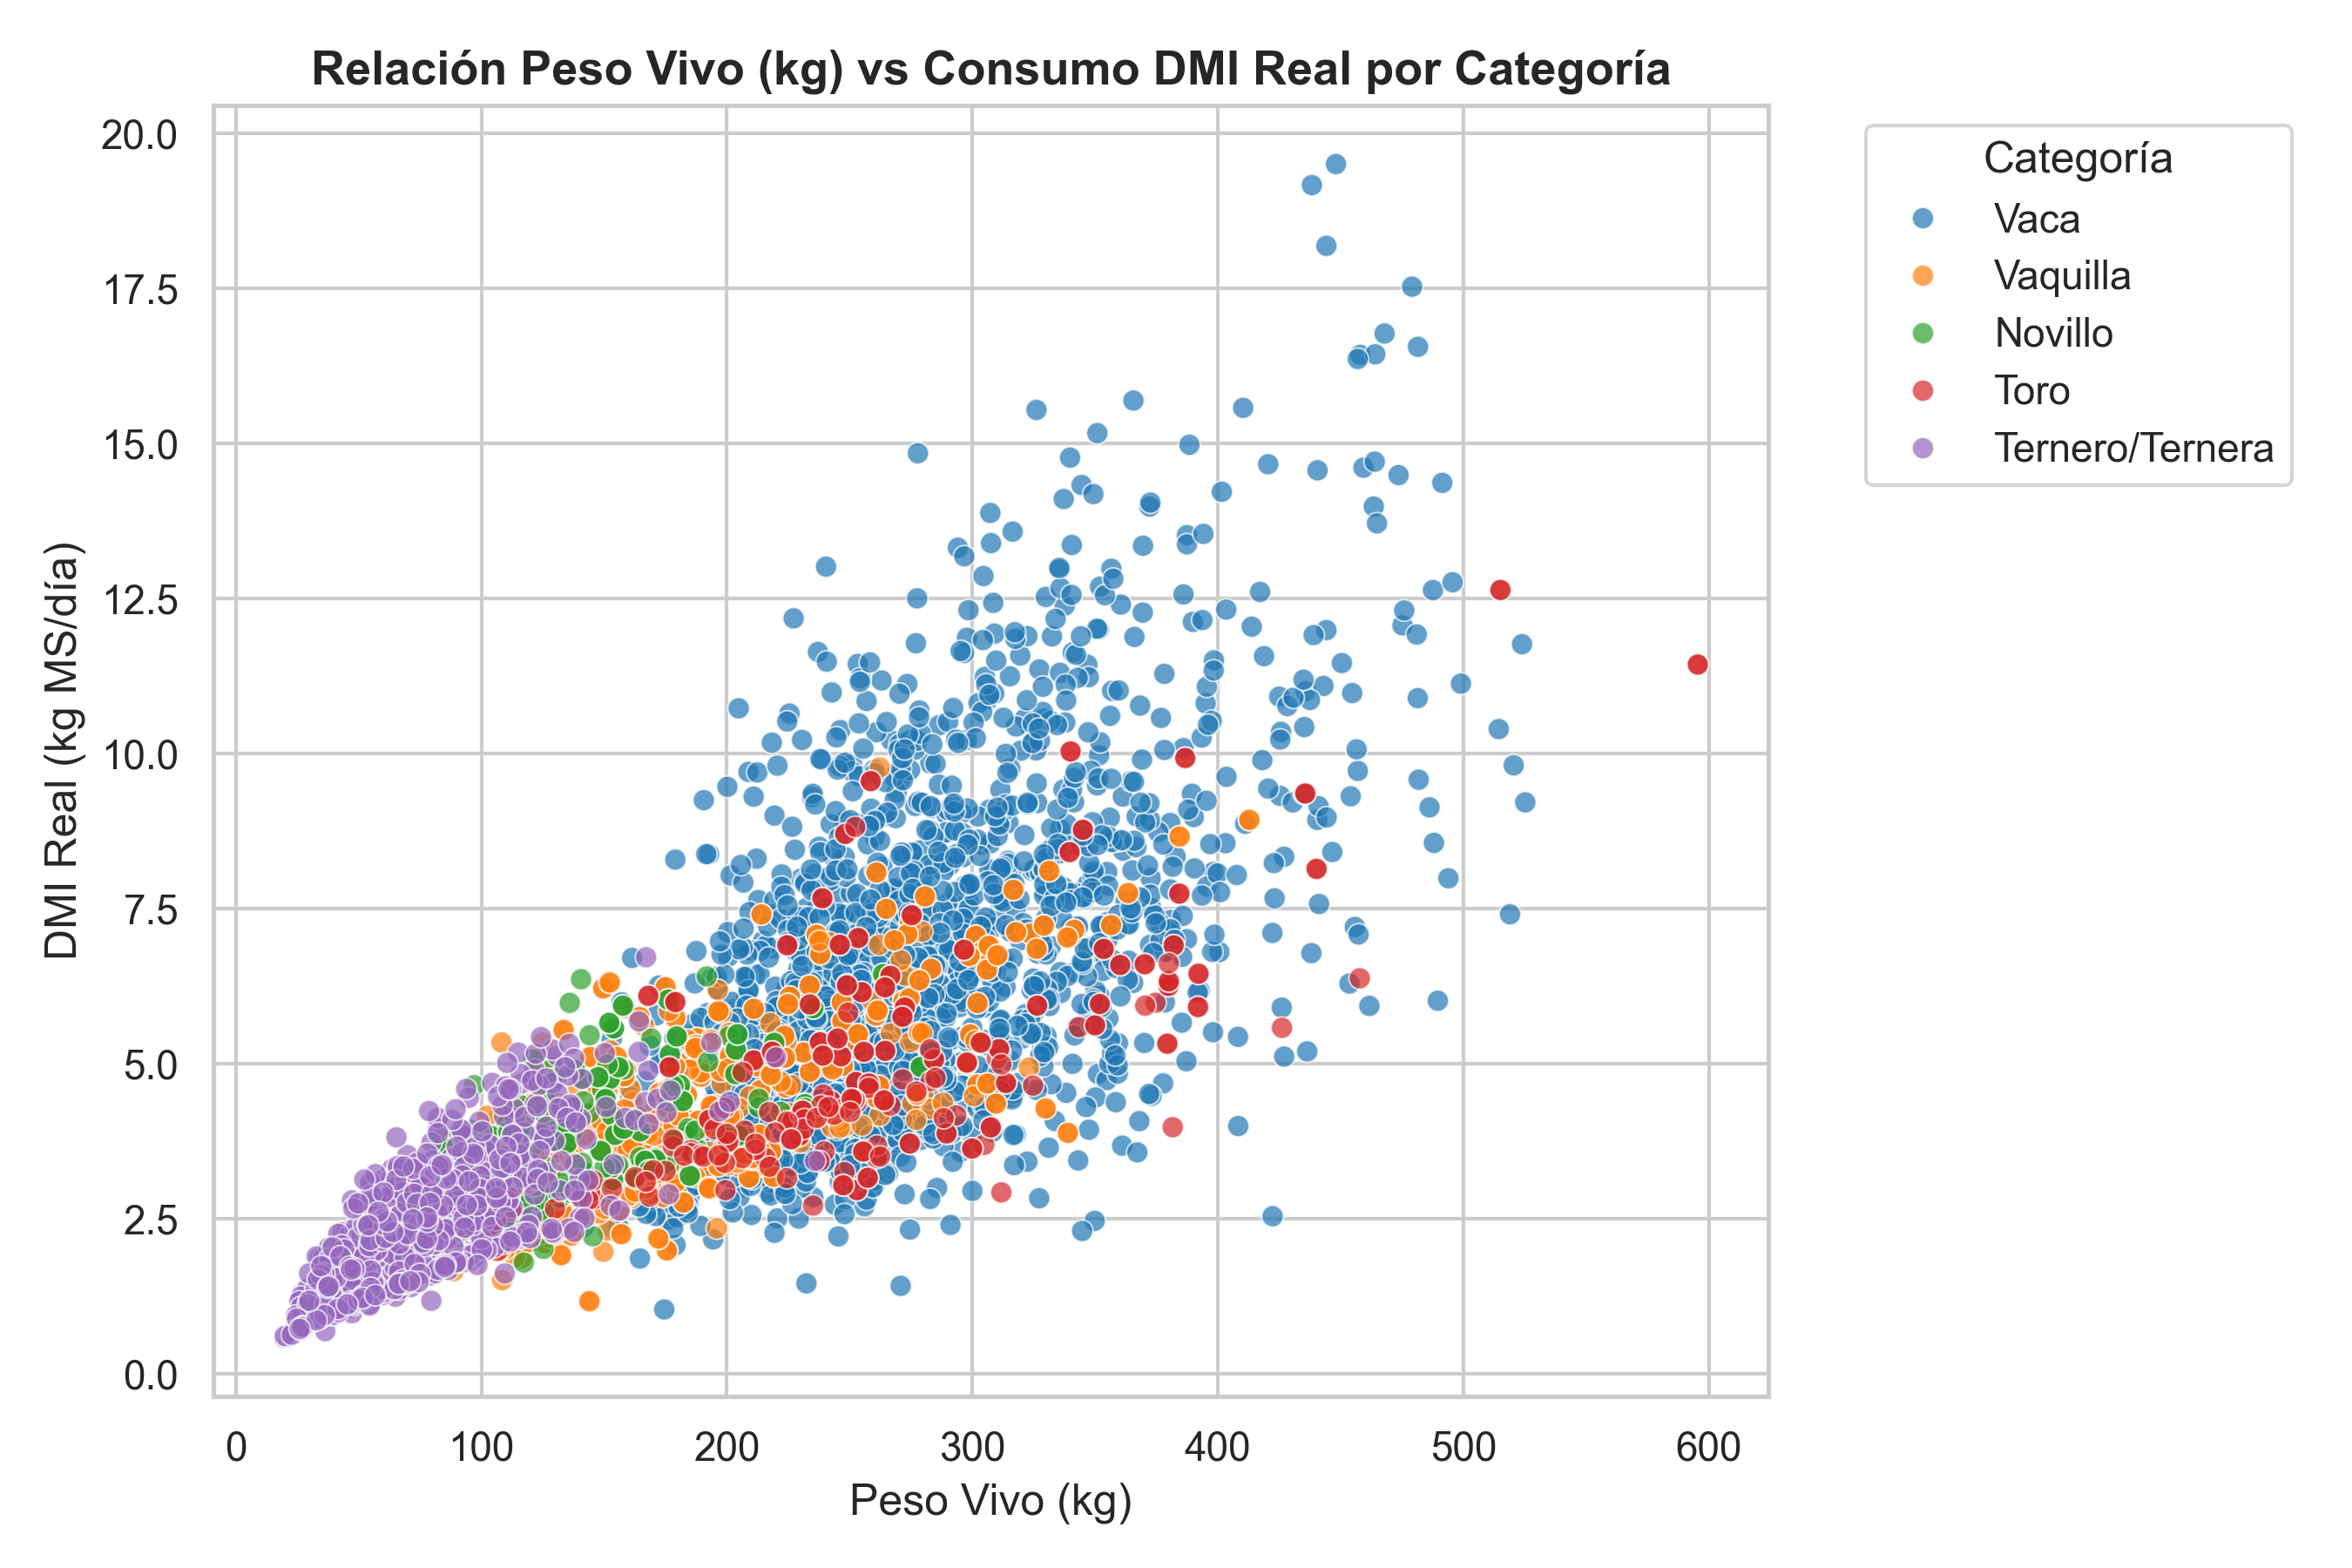
\includegraphics[width=0.9\textwidth]{figures/6_weight_vs_dmi_scatter.png}
\caption{Relación observada entre peso vivo y DMI, diferenciada por categoría. La asociación positiva fundamenta la capacidad predictiva del peso, pero no demuestra causalidad por sí sola.}
\end{figure}

\begin{figure}[H]
\centering
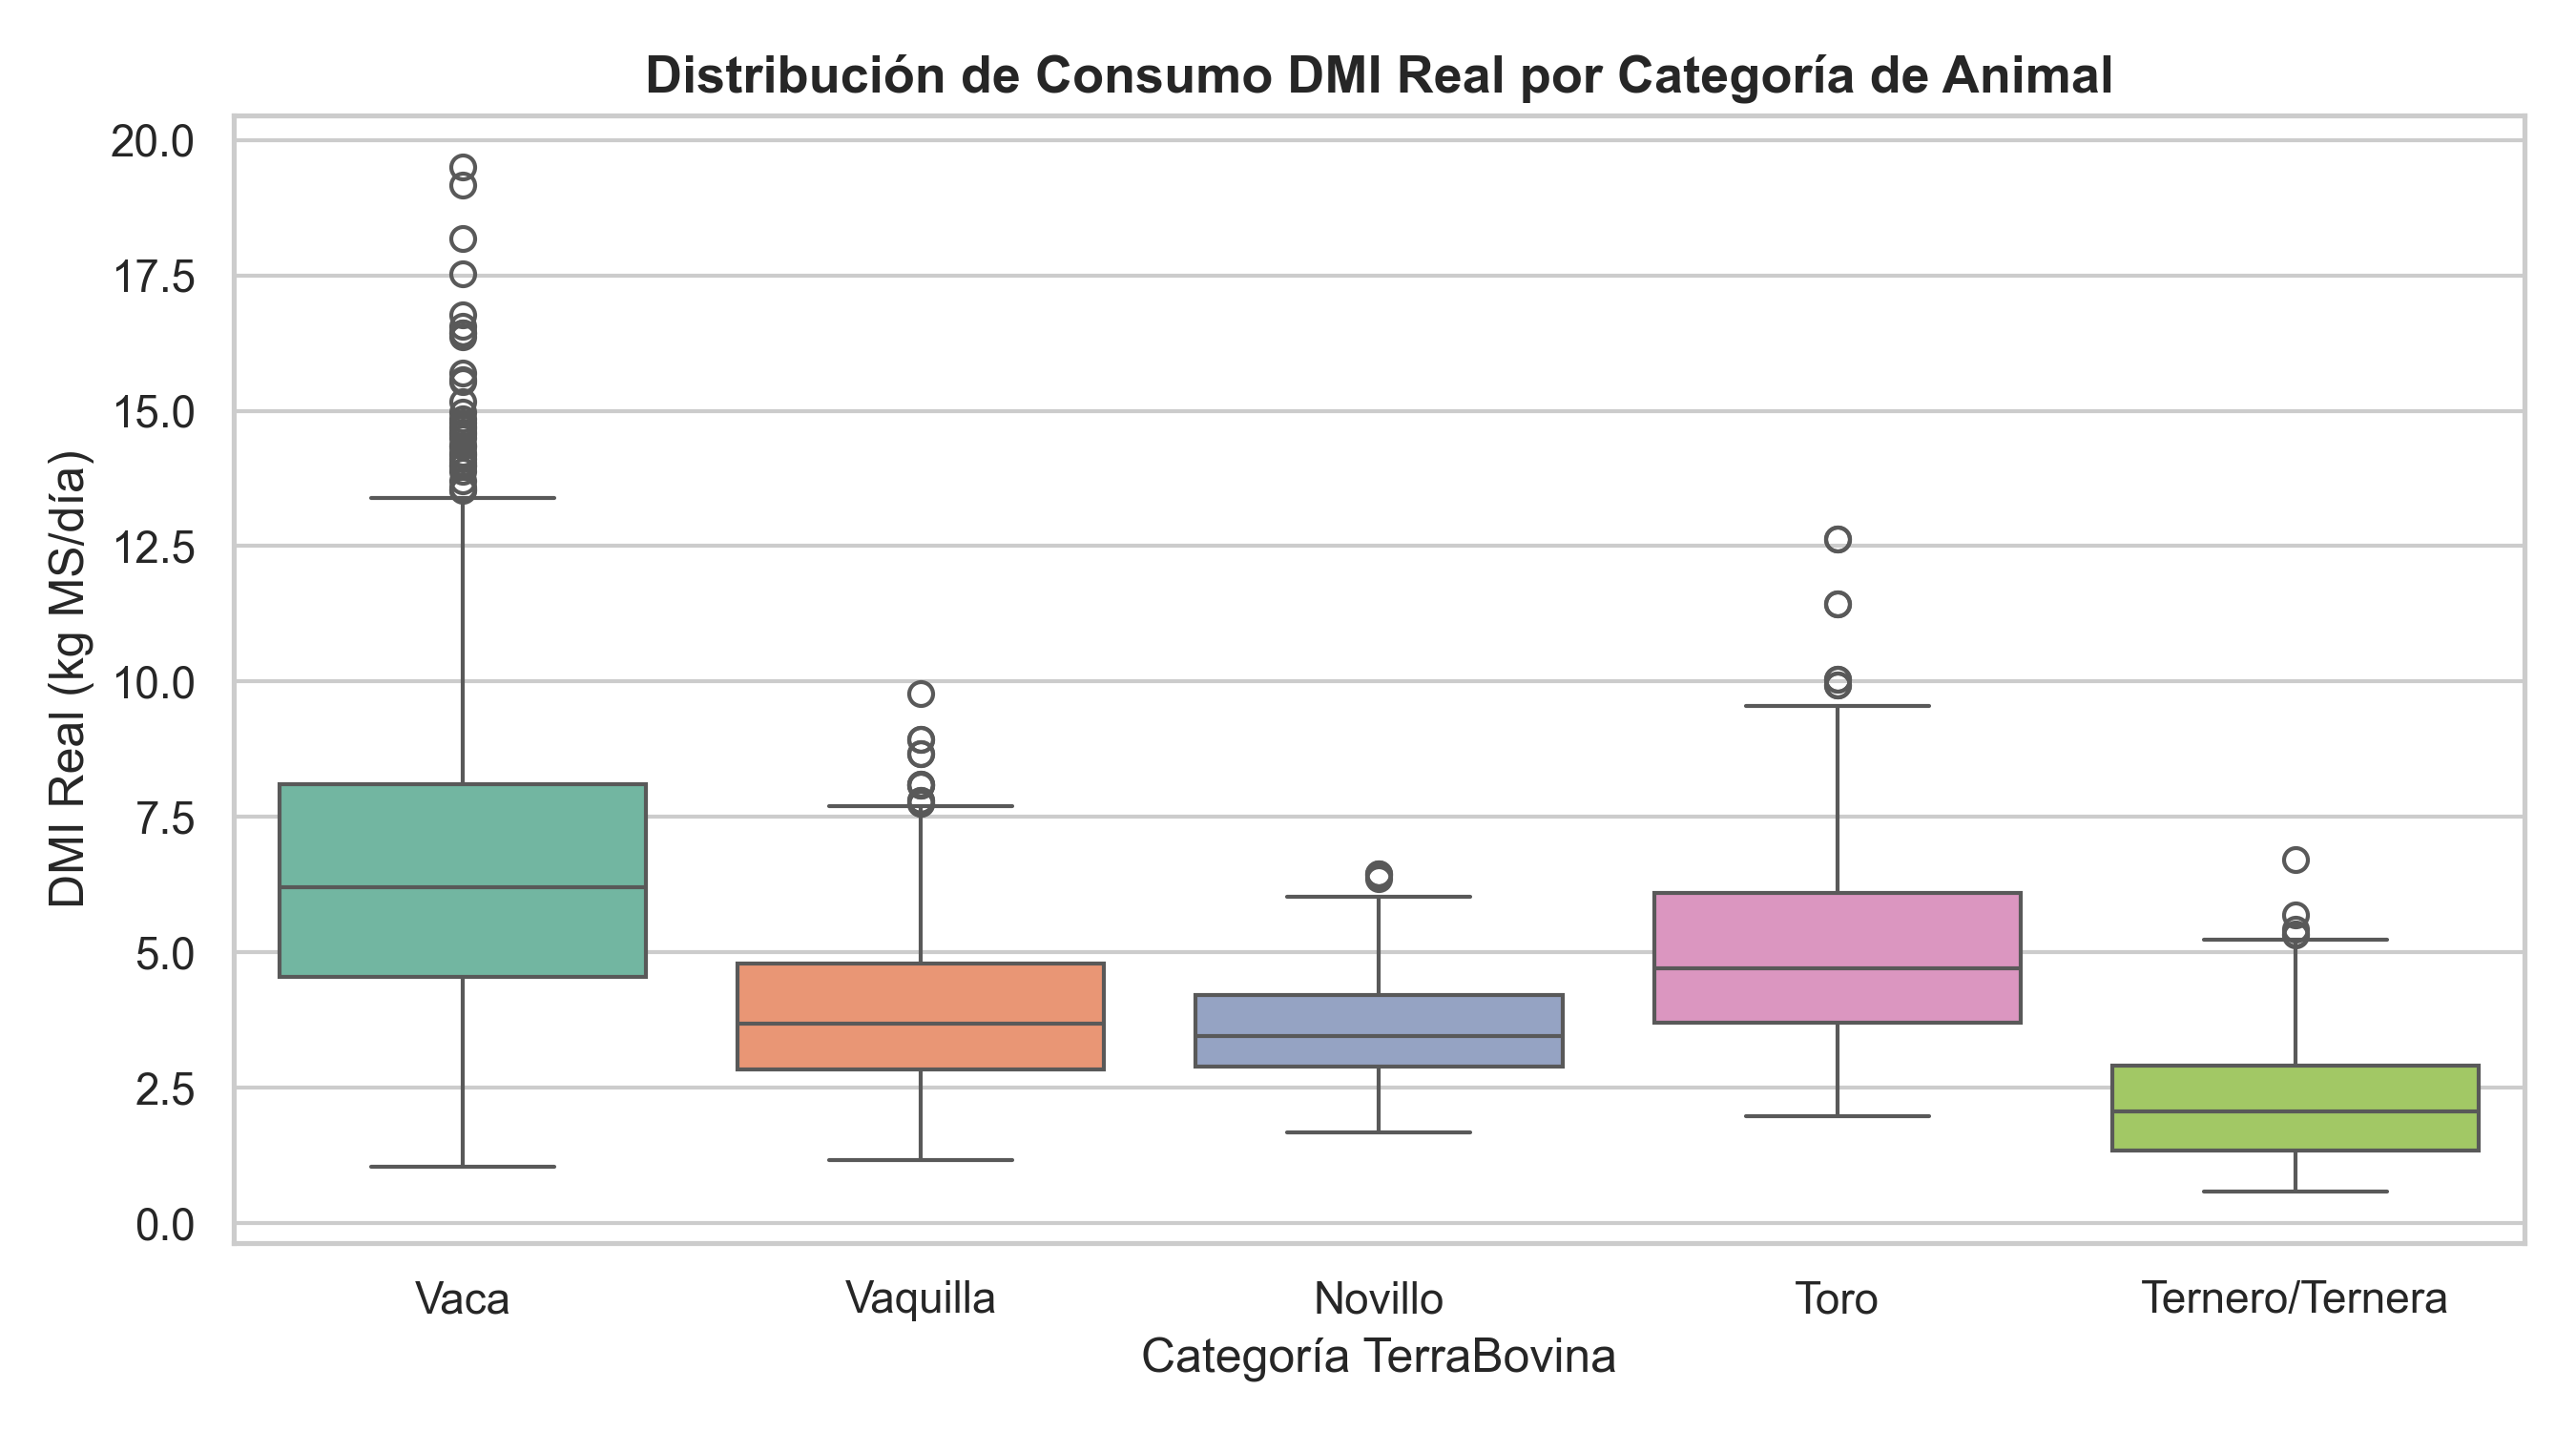
\includegraphics[width=0.9\textwidth]{figures/7_dmi_by_category_boxplot.png}
\caption{Distribución del DMI por categoría. Las vacas presentan mayor dispersión, lo que contribuye a su mayor error absoluto.}
\end{figure}

\section{Proceso ETL}

ETL significa extracción, transformación y carga. La implementación divide cada etapa en un módulo para facilitar mantenimiento y prueba.

\subsection{Extracción}

\archivo{src/etl/extract.py} verifica la existencia física de la fuente, la lee con \archivo{pandas.read_csv} y exige siete columnas contractuales: identificador, hogar, categoría, peso, DMI, condición corporal y estado fisiológico. Si falta una columna o el archivo no existe, la ejecución se detiene. También registra dimensiones y nulos iniciales.

\subsection{Transformación}

\archivo{transform_data} realiza, en orden, las siguientes operaciones:
\begin{enumerate}
  \item Copia el DataFrame para no modificar accidentalmente el argumento.
  \item Combina las banderas \archivo{outlier_peso}, \archivo{outlier_dmi_abs} y \archivo{outlier_dmi_pct_bw}; elimina una fila si cualquiera es verdadera.
  \item Convierte peso, DMI y condición corporal con \archivo{pd.to_numeric(errors="coerce")}; entradas inválidas pasan a nulo.
  \item Elimina espacios en categorías y normaliza estados a mayúsculas; nulos o cadenas vacías se convierten en DESCONOCIDO.
  \item Conserva pesos entre 15 y 900 kg, DMI entre 0,2 y 20 kg/día y las cinco categorías oficiales.
  \item Para animales que no son vacas, asigna condición corporal nula y estado DESCONOCIDO.
  \item Recalcula el porcentaje de DMI sobre peso vivo.
  \item Calcula metadatos de retención y estadísticas por categoría.
\end{enumerate}

\subsection{Carga y orquestación}

\archivo{load_data} crea los directorios necesarios, guarda el CSV sin índice y escribe el resumen ETL en JSON. \archivo{run_etl_pipeline} elige el CSV crudo si existe; si no existe, utiliza como fuente el propio CSV procesado. En el estado actual no existe \archivo{data/raw/terrabovina_dmi_kenya_raw.csv}; por eso el reporte disponible describe una ejecución 3.833 $\rightarrow$ 3.833 con retención del 100\%, no la limpieza histórica original.

Este fallback permite ejecutar el flujo, pero debilita la trazabilidad y puede sobrescribir el único dataset conservado. Para una entrega productiva convendría exigir una fuente cruda inmutable y escribir un archivo procesado versionado.

\section{Preparación de características}

\archivo{src/model/features.py} concentra las constantes compartidas:
\begin{itemize}
  \item Objetivo: \archivo{dmi_kg_dia}.
  \item Grupo: \archivo{hh}.
  \item Numéricas: \archivo{peso_vivo_kg}, \archivo{condicion_corporal}.
  \item Categóricas: \archivo{categoria_terrabovina}, \archivo{estado_fisiologico_norm}.
\end{itemize}

\archivo{prepare_features} verifica las entradas, selecciona únicamente esas cuatro columnas, exige peso numérico, convierte condición inválida a nulo y normaliza texto. La misma función se usa al entrenar y predecir, lo cual evita diferencias entre ambos entornos. Para no vacas vuelve a imponer condición nula y estado DESCONOCIDO.

\archivo{load_training_data} exige entradas, objetivo y grupo; rechaza datasets con menos de 1.000 filas; prepara $X$, $y$ y \archivo{groups}; y comprueba rangos globales de DMI y peso. No valida de forma explícita categorías desconocidas, unicidad, fechas, tamaño mínimo por subgrupo ni consistencia temporal.

\subsection{Pipeline de scikit-learn}

Para Ridge y Random Forest se usa un \archivo{ColumnTransformer}:
\begin{itemize}
  \item \textbf{Numéricas:} \archivo{SimpleImputer(strategy="median", add_indicator=True)} y luego \archivo{StandardScaler}. La mediana es robusta frente a extremos y el indicador informa al modelo si el valor estaba ausente.
  \item \textbf{Categóricas:} \archivo{OneHotEncoder(handle_unknown="ignore", sparse_output=False)}. Cada nivel se convierte en una columna binaria; un nivel desconocido no detiene el proceso, sino que produce ceros en ese bloque.
\end{itemize}

El escalado transforma cada variable aproximadamente como
\begin{equation}
z=\frac{x-\mu}{\sigma}.
\end{equation}
Es especialmente importante para Ridge, porque la penalización debe actuar sobre escalas comparables.

\begin{figure}[H]
\centering
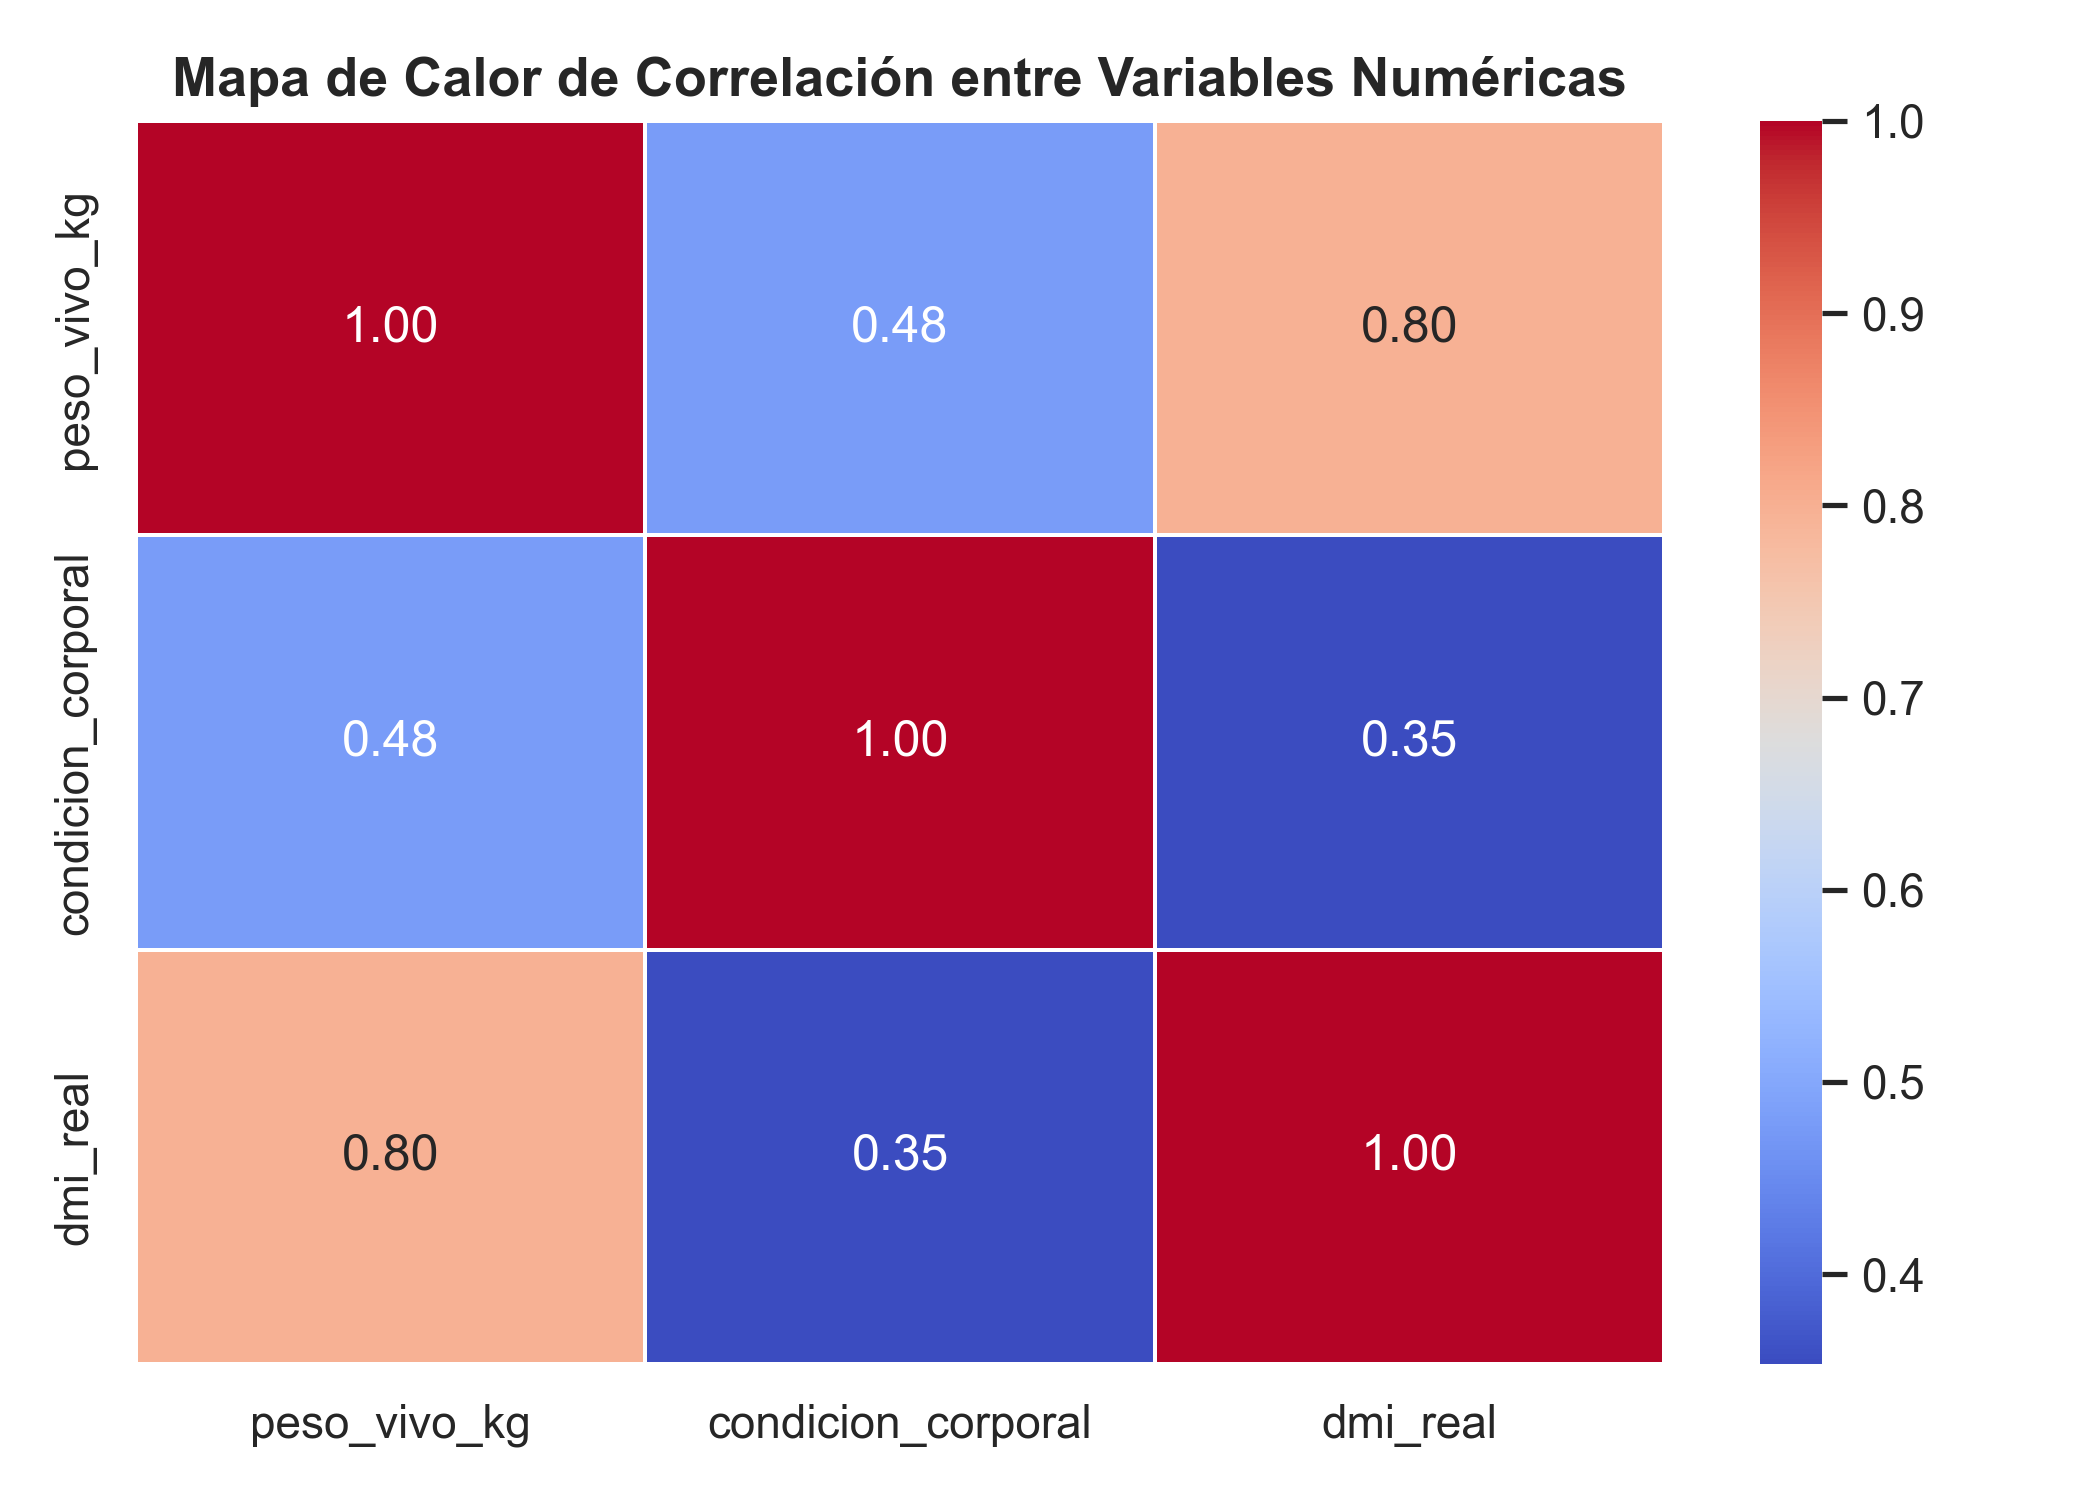
\includegraphics[width=0.75\textwidth]{figures/8_correlation_heatmap.png}
\caption{Correlaciones lineales entre variables numéricas preparadas y DMI. Correlación no equivale a causalidad y no captura relaciones no lineales.}
\end{figure}

\section{Modelos evaluados}

\subsection{Baseline de la media}

\archivo{DummyRegressor(strategy="mean")} predice en cada fold la media del objetivo de entrenamiento. No pretende ser competitivo: fija un nivel mínimo. Si un modelo complejo no lo supera, las características o el procedimiento no aportan capacidad predictiva útil.

\subsection{Regresión Ridge}

Ridge minimiza la suma de errores cuadrados más una penalización L2:
\begin{equation}
\min_{\beta_0,\boldsymbol{\beta}}\sum_{i=1}^{n}(y_i-\beta_0-\mathbf{x}_i^T\boldsymbol{\beta})^2+\alpha\sum_{j=1}^{p}\beta_j^2.
\end{equation}
Con $\alpha=10$, la penalización contrae coeficientes y reduce varianza frente a una regresión lineal sin regularización. No los lleva necesariamente a cero. Es apropiado cuando la señal es aproximadamente aditiva y lineal y existen variables one-hot correlacionadas.

\subsection{Random Forest}

Un bosque aleatorio promedia múltiples árboles de decisión entrenados con aleatoriedad en muestras y variables. Puede capturar umbrales, interacciones y relaciones no lineales sin especificarlas manualmente. Se configuran 100 árboles, profundidad máxima 10 y semilla 42. Su desventaja es menor interpretabilidad y una función predictiva por regiones; además, los árboles no extrapolan tendencias lineales fuera del rango observado.

\subsection{CatBoost}

CatBoost es un método de gradient boosting: agrega árboles secuencialmente para corregir errores residuales. Está diseñado para manejar variables categóricas y reducir sesgos asociados a su codificación. Se ejecuta con 500 iteraciones, profundidad 6, tasa de aprendizaje 0,04, pérdida RMSE, semilla 42 y escritura de archivos desactivada.

\begin{table}[H]
\centering
\caption{Configuración exacta de candidatos.}
\begin{tabularx}{\textwidth}{p{3cm}X}
\toprule
\textbf{Modelo} & \textbf{Parámetros definidos explícitamente}\\
\midrule
Baseline & \archivo{strategy="mean"}.\\
Ridge & \archivo{alpha=10.0}; demás parámetros de la versión instalada.\\
Random Forest & \archivo{n_estimators=100}, \archivo{max_depth=10}, \archivo{random_state=42}.\\
CatBoost & \archivo{iterations=500}, \archivo{depth=6}, \archivo{learning_rate=0.04}, \archivo{loss_function="RMSE"}, variables categóricas declaradas, \archivo{random_seed=42}, \archivo{verbose=False}, \archivo{allow_writing_files=False}.\\
\bottomrule
\end{tabularx}
\end{table}

No hay búsqueda de hiperparámetros ni validación anidada. Los valores están fijados manualmente en el código. Por tanto, la comparación describe esas configuraciones concretas, no el máximo rendimiento posible de cada familia.

\section{Diseño de validación y entrenamiento}

\subsection{StratifiedGroupKFold}

Se utilizan cinco folds, mezcla activada y semilla 42. La estratificación intenta mantener la proporción de categorías y el agrupamiento por \archivo{hh} obliga a que un hogar aparezca enteramente en entrenamiento o en prueba. El código verifica explícitamente que la intersección de hogares sea vacía y detiene el proceso si detecta fuga.

En cada candidato se genera un vector \textit{out-of-fold}: cada registro recibe una predicción producida por un modelo que no fue entrenado con ese fold. Estas predicciones se usan para métricas y gráficos. Después de predecir, los valores negativos se truncan a cero, una restricción coherente con el dominio físico aunque no forme parte del ajuste de Ridge.

Se realizan $4\times5=20$ ajustes de evaluación. El ganador es el nombre con menor MAE global; luego se realiza un ajuste final sobre las 3.833 filas, totalizando 21 ajustes. El ajuste final maximiza datos para inferencia, pero ya no sirve para medir rendimiento: la estimación de generalización es la validación cruzada.

\subsection{Métricas}

El error de una observación es $e_i=y_i-\hat y_i$.

\textbf{MAE:}
\begin{equation}
MAE=\frac{1}{n}\sum_{i=1}^{n}|y_i-\hat y_i|.
\end{equation}
Está en kg MS/día y representa el error absoluto promedio. Es fácil de interpretar y menos sensible a errores extremos que RMSE. Es la métrica de selección.

\textbf{RMSE:}
\begin{equation}
RMSE=\sqrt{\frac{1}{n}\sum_{i=1}^{n}(y_i-\hat y_i)^2}.
\end{equation}
También está en kg MS/día, pero penaliza más los errores grandes. Que RMSE sea mayor que MAE indica la presencia de errores de magnitud elevada.

\textbf{Coeficiente de determinación:}
\begin{equation}
R^2=1-\frac{\sum_i(y_i-\hat y_i)^2}{\sum_i(y_i-\bar y)^2}.
\end{equation}
Un valor 1 indica ajuste perfecto; 0 equivale aproximadamente a predecir la media bajo la misma muestra; puede ser negativo cuando se rinde peor. No expresa porcentaje de predicciones correctas y no mide error en kilogramos.

\section{Resultados y comparación}

\begin{table}[H]
\centering
\caption{Resultados globales sobre predicciones out-of-fold.}
\begin{tabular}{lrrr}
\toprule
\textbf{Modelo} & \textbf{MAE} & \textbf{RMSE} & \textbf{$R^2$}\\
\midrule
Baseline media & 2,1280 & 2,7273 & -0,0029\\
\textbf{Ridge} & \textbf{1,1019} & \textbf{1,5354} & \textbf{0,6821}\\
Random Forest & 1,1611 & 1,6458 & 0,6348\\
CatBoost & 1,1027 & 1,5587 & 0,6724\\
\bottomrule
\end{tabular}
\end{table}

Ridge reduce el MAE frente al baseline en aproximadamente
\begin{equation}
\frac{2,1280-1,1019}{2,1280}\times100\approx48,2\%.
\end{equation}
La mejora confirma que las variables aportan señal. Ridge también presenta el menor RMSE y el mayor $R^2$. Sin embargo, su diferencia de MAE frente a CatBoost es 0,0008 kg/día, menos de un gramo de materia seca por día en el valor agregado de la métrica. Sin intervalos de confianza, repeticiones con otras semillas ni comparación pareada por hogar, no puede afirmarse que esa ventaja sea estable.

\begin{figure}[H]
\centering
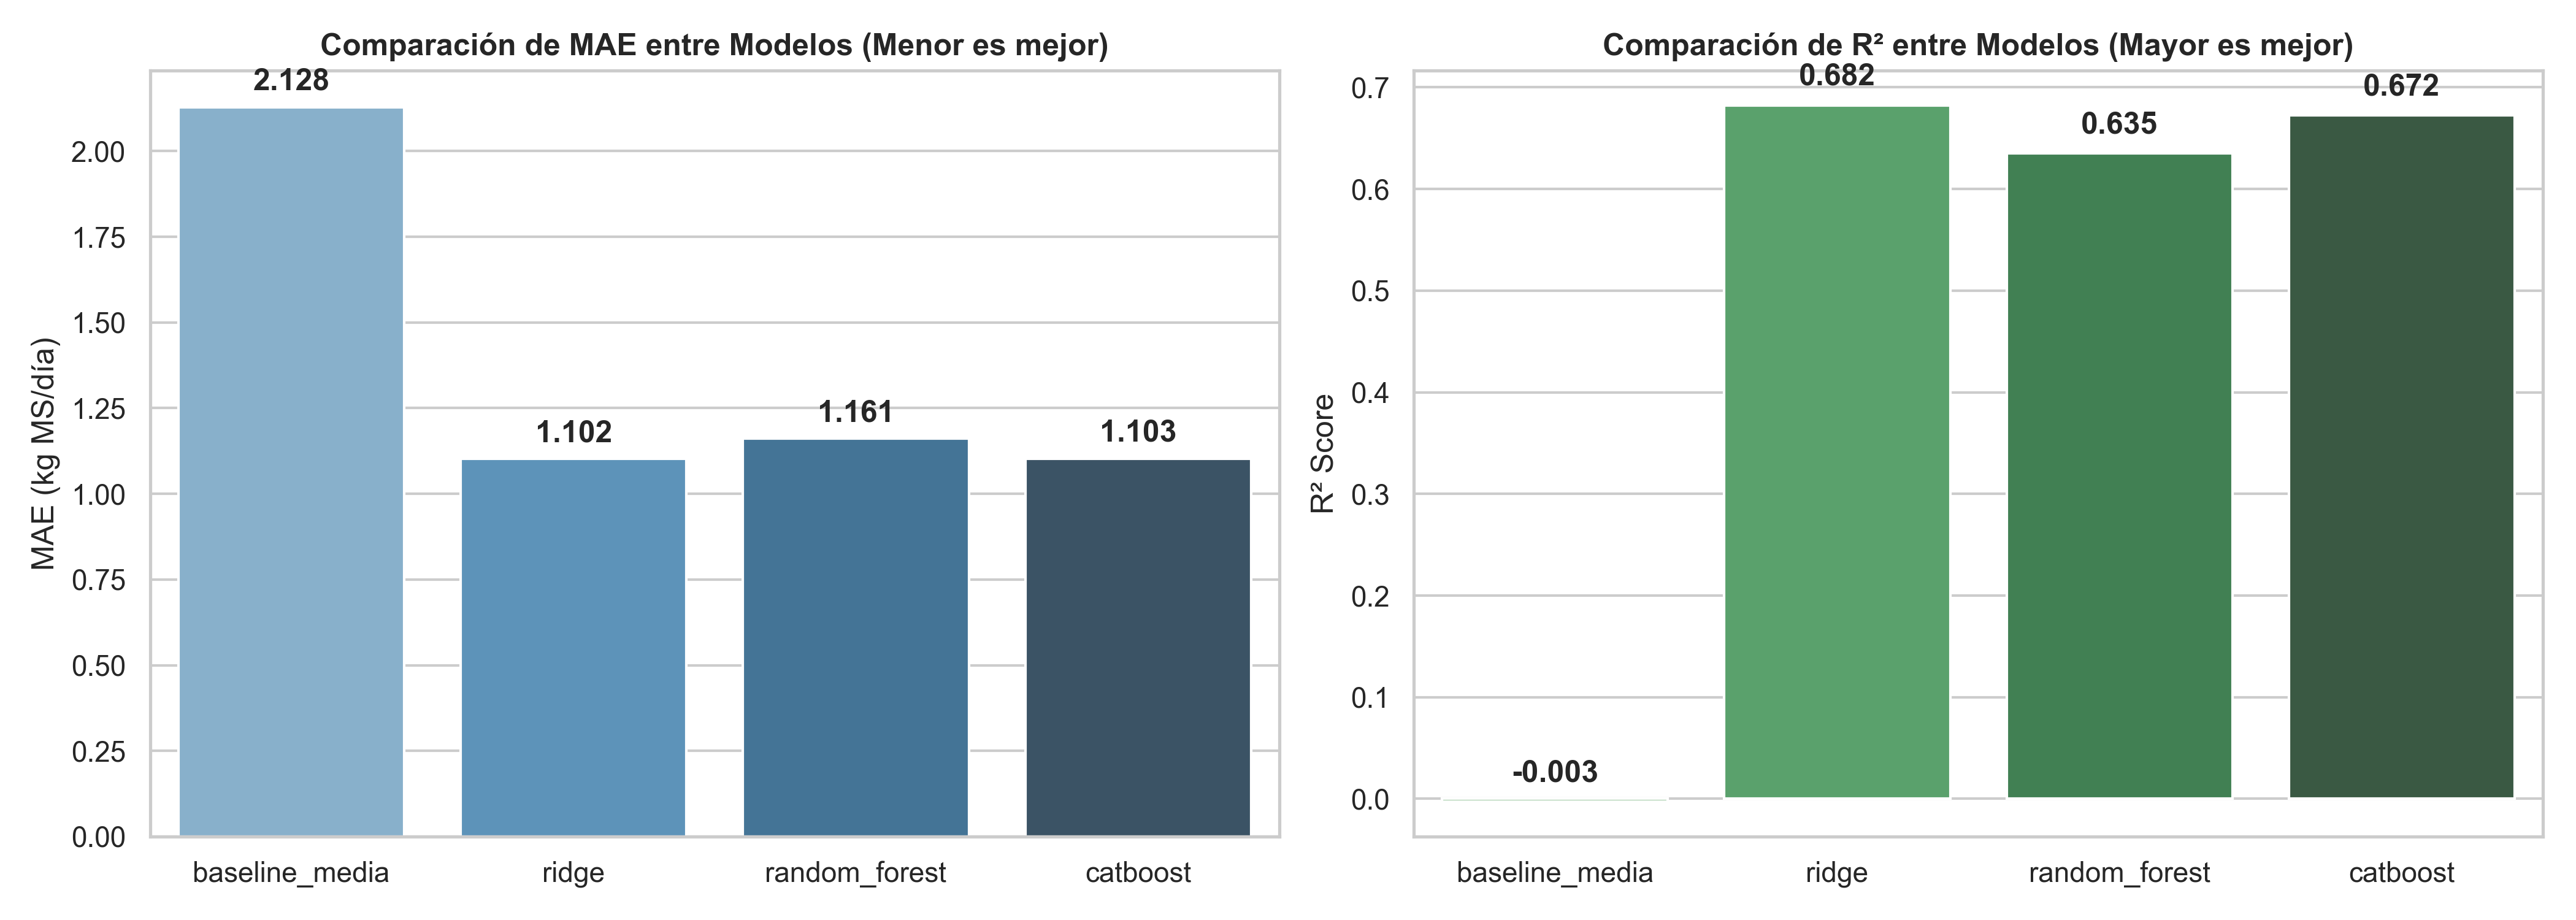
\includegraphics[width=\textwidth]{figures/1_model_comparison_mae_r2.png}
\caption{Comparación global. El baseline queda claramente rezagado; Ridge y CatBoost resultan prácticamente equivalentes en MAE.}
\end{figure}

\subsection{Estabilidad por fold}

\begin{table}[H]
\centering
\caption{Resultados de Ridge en los cinco folds.}
\begin{tabular}{crrr}
\toprule
\textbf{Fold} & \textbf{MAE} & \textbf{RMSE} & \textbf{$R^2$}\\
\midrule
1 & 1,1138 & 1,5369 & 0,6617\\
2 & 1,0993 & 1,5368 & 0,7214\\
3 & 1,1558 & 1,6039 & 0,6830\\
4 & 1,0742 & 1,4878 & 0,6818\\
5 & 1,0715 & 1,5164 & 0,6314\\
\bottomrule
\end{tabular}
\end{table}

El MAE oscila entre 1,0715 y 1,1558, rango de 0,0843 kg/día. El $R^2$ varía entre 0,6314 y 0,7214. Esto sugiere consistencia razonable entre particiones, aunque cinco valores no sustituyen intervalos de confianza ni validación externa.

\subsection{Resultados por categoría}

\begin{table}[H]
\centering
\caption{Métricas de Ridge por categoría.}
\begin{tabular}{lrrr}
\toprule
\textbf{Categoría} & \textbf{MAE} & \textbf{RMSE} & \textbf{$R^2$}\\
\midrule
Vaca & 1,5857 & 2,0608 & 0,4110\\
Vaquilla & 0,7540 & 0,9449 & 0,6037\\
Novillo & 0,6639 & 0,8028 & 0,4126\\
Toro & 1,0204 & 1,3642 & 0,5068\\
Ternero/Ternera & 0,5846 & 0,7018 & 0,5858\\
\bottomrule
\end{tabular}
\end{table}

El mayor MAE corresponde a vacas. Parte de la diferencia es de escala: las vacas consumen más y presentan mayor dispersión. Esto evidencia por qué una métrica global no basta. CatBoost logra mejor resultado que Ridge en Ternero/Ternera, y Random Forest lo supera levemente en Novillo; el ganador global no domina todos los subgrupos.

\begin{figure}[H]
\centering
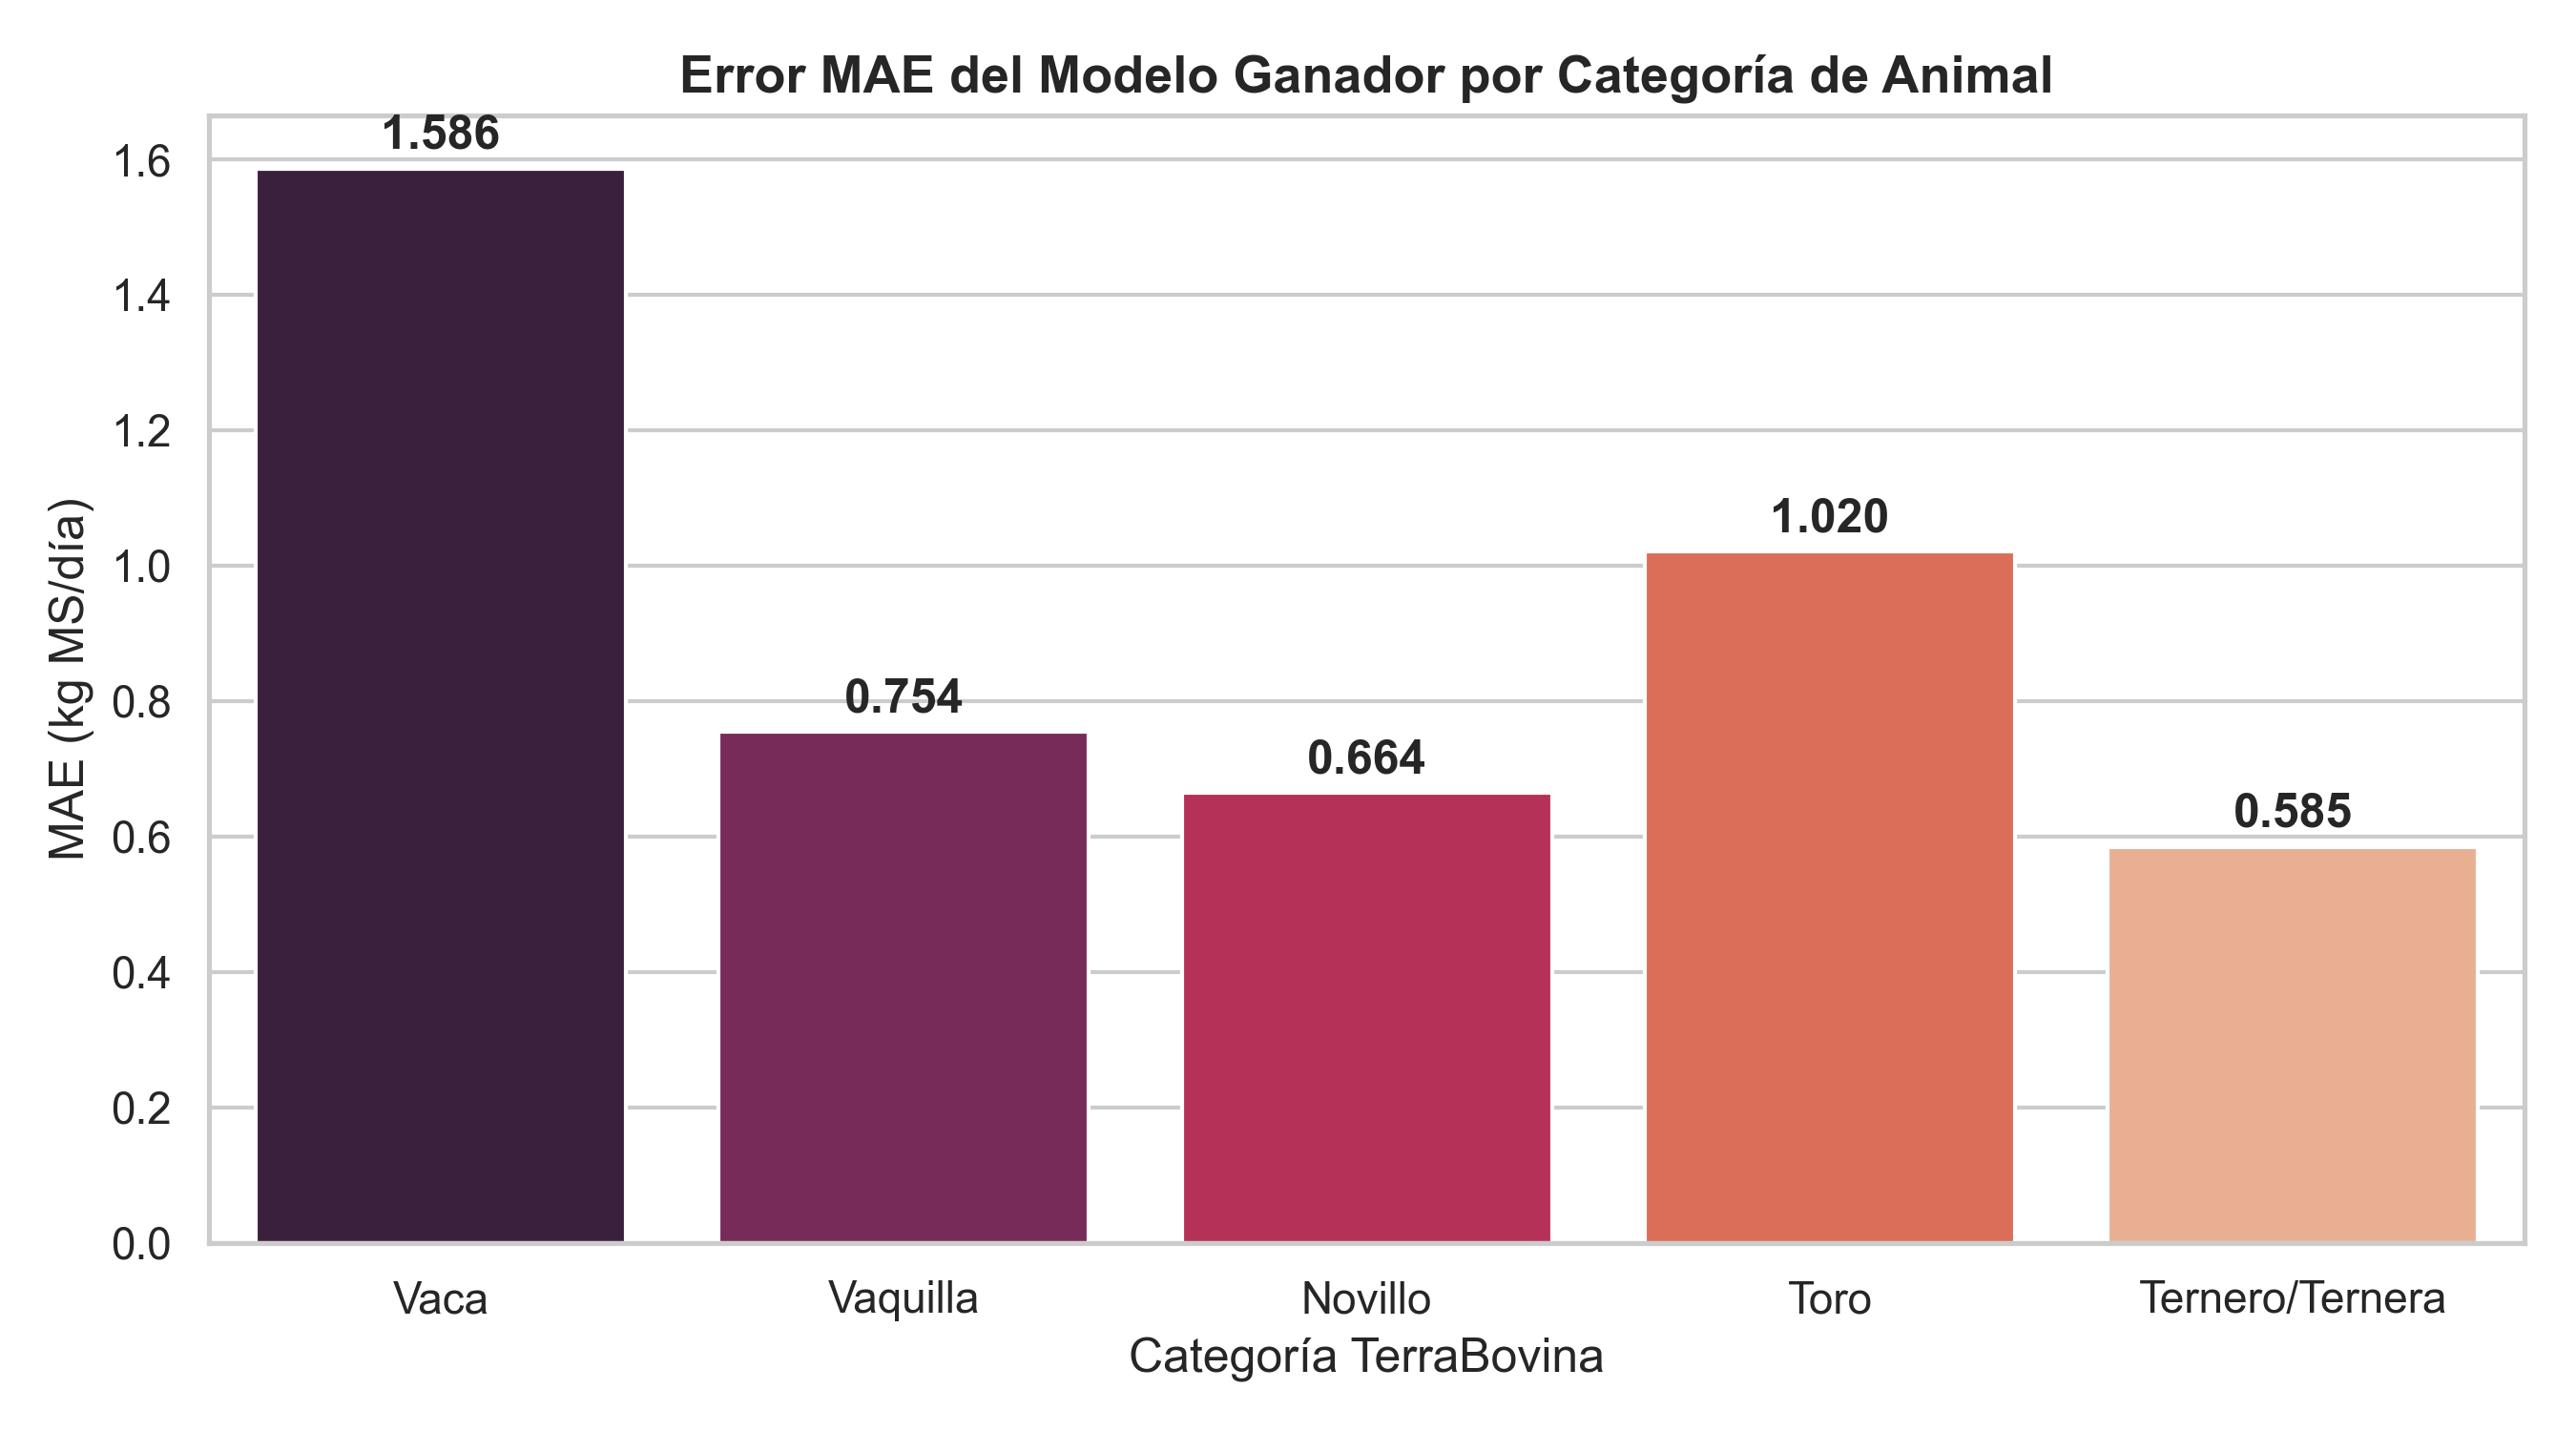
\includegraphics[width=0.9\textwidth]{figures/5_mae_by_category.png}
\caption{MAE del modelo ganador por categoría. El error absoluto no debe compararse sin considerar escala y variabilidad del DMI en cada grupo.}
\end{figure}

\subsection{Predicción, ajuste y residuos}

\begin{figure}[H]
\centering
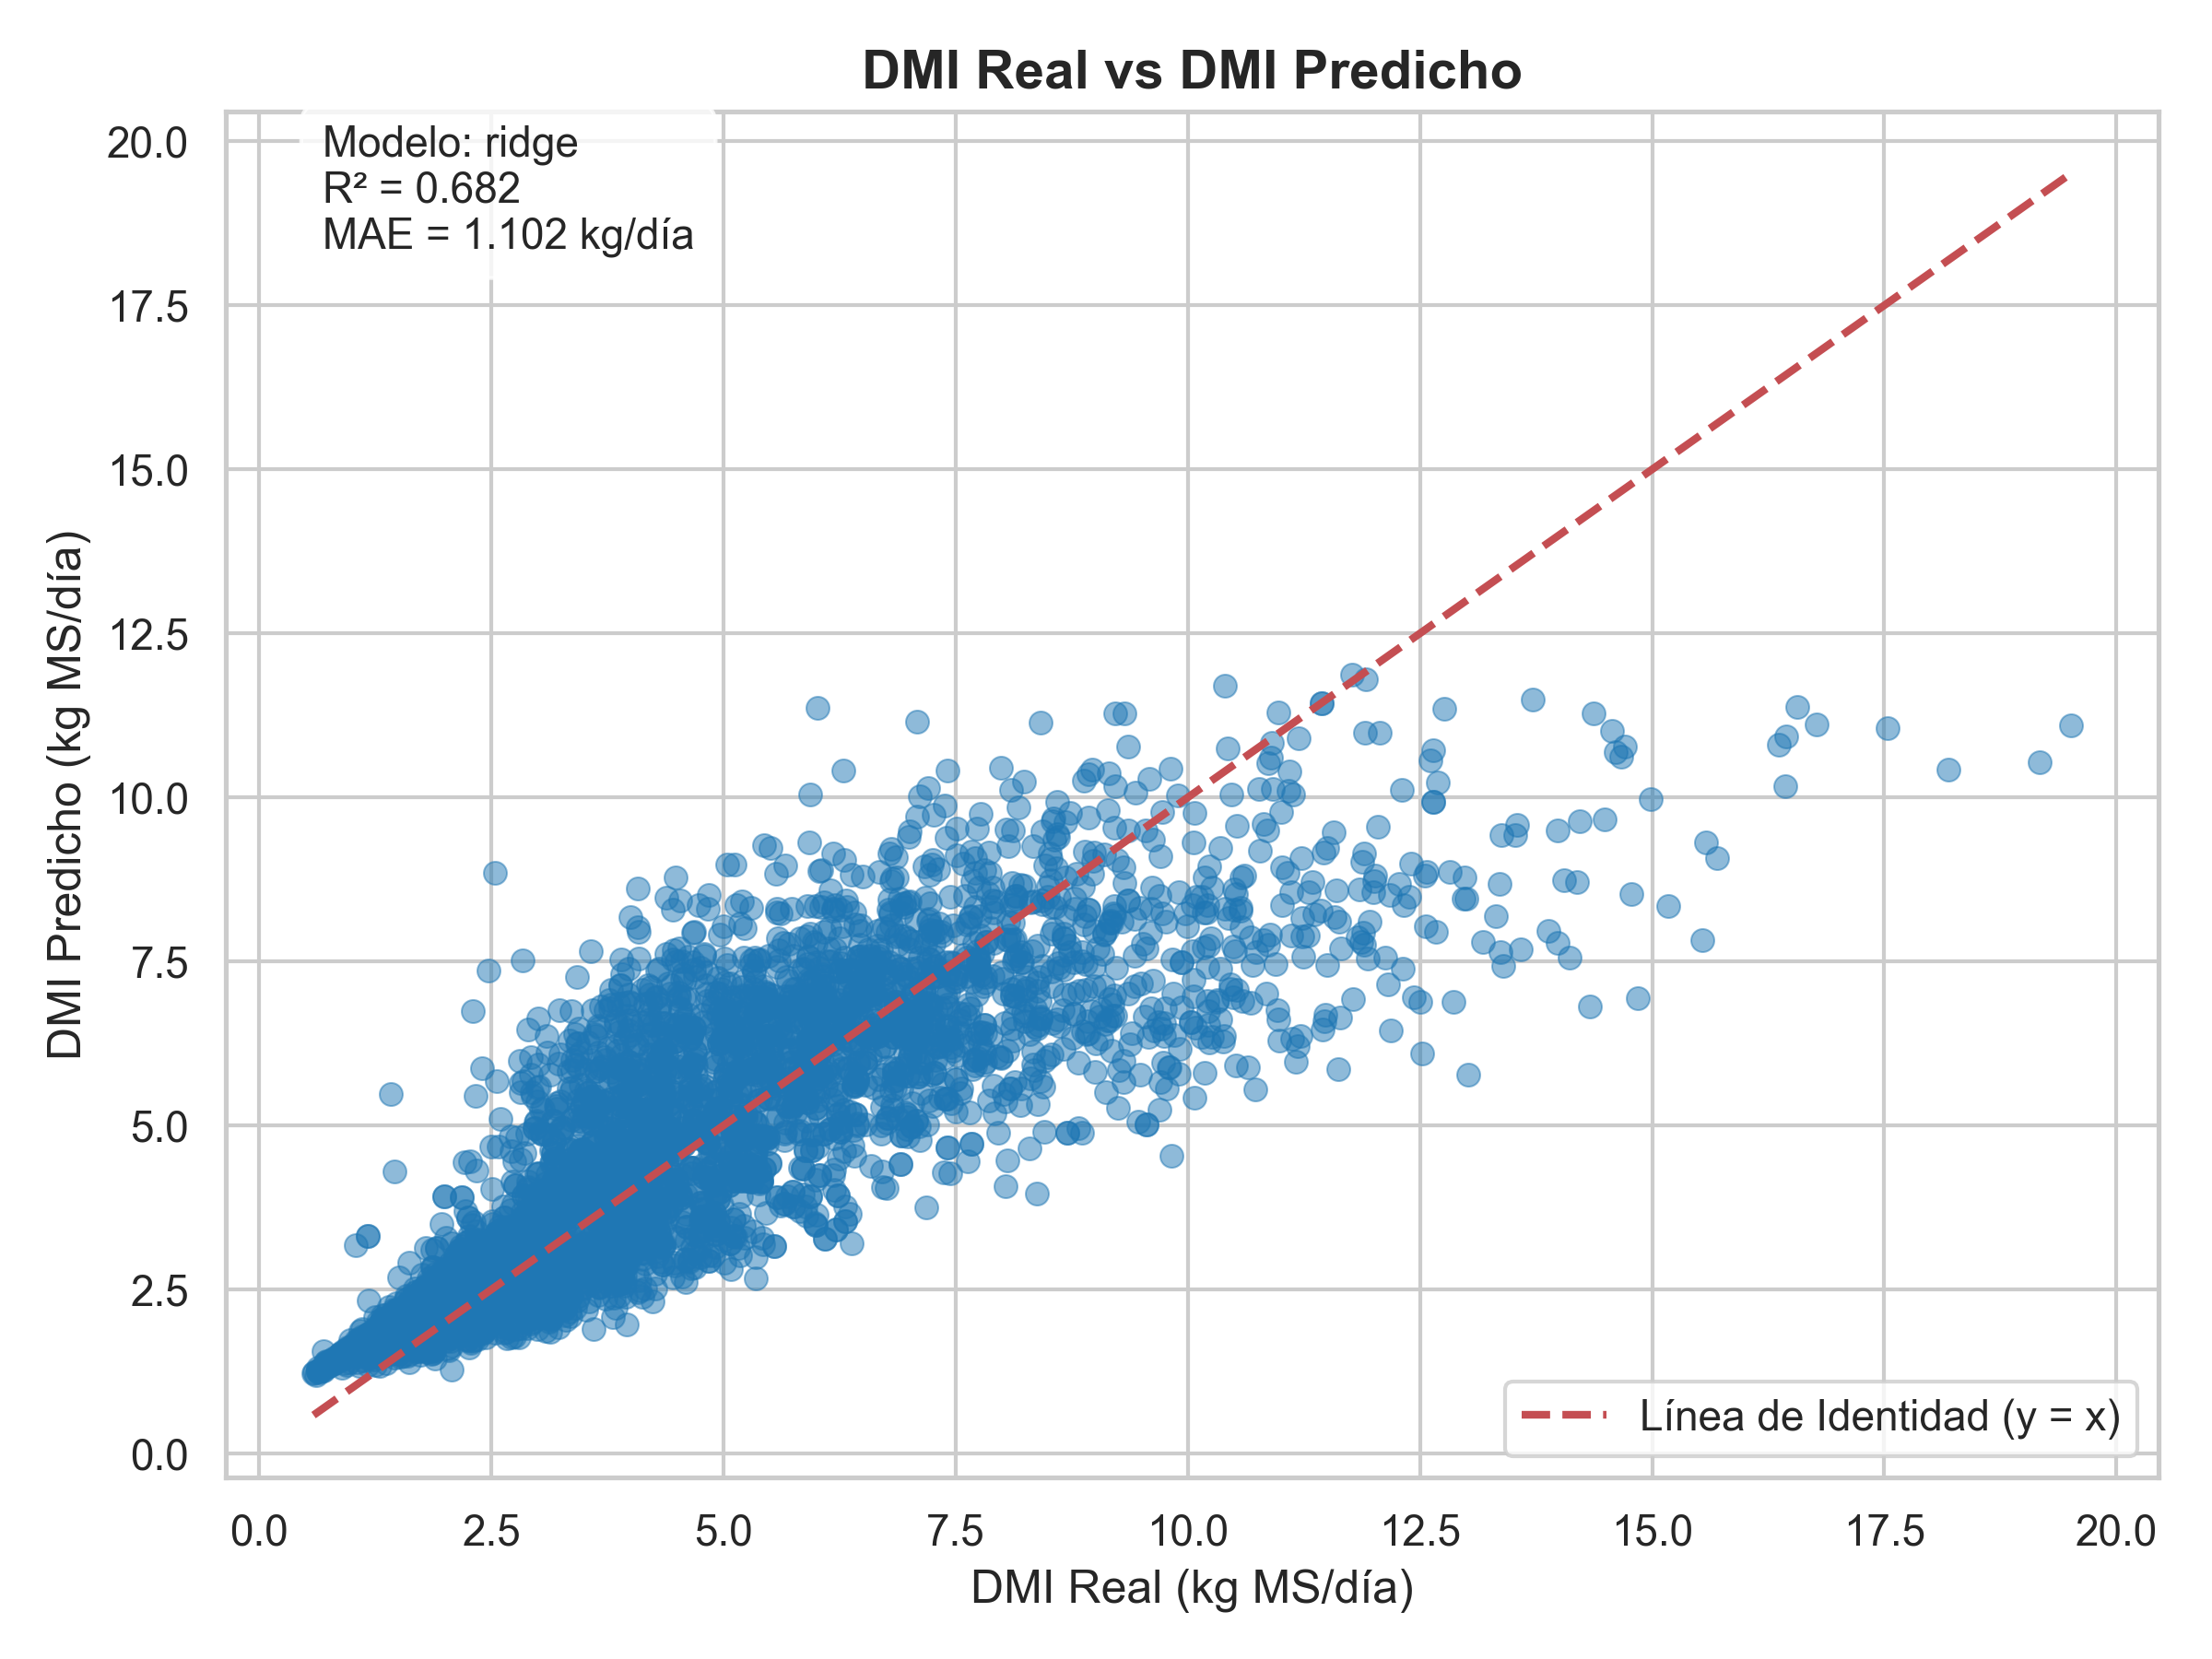
\includegraphics[width=0.82\textwidth]{figures/2_actual_vs_predicted.png}
\caption{DMI real frente a predicho mediante estimaciones out-of-fold. La diagonal representa predicción perfecta; la dispersión alrededor de ella representa error.}
\end{figure}

\begin{figure}[H]
\centering
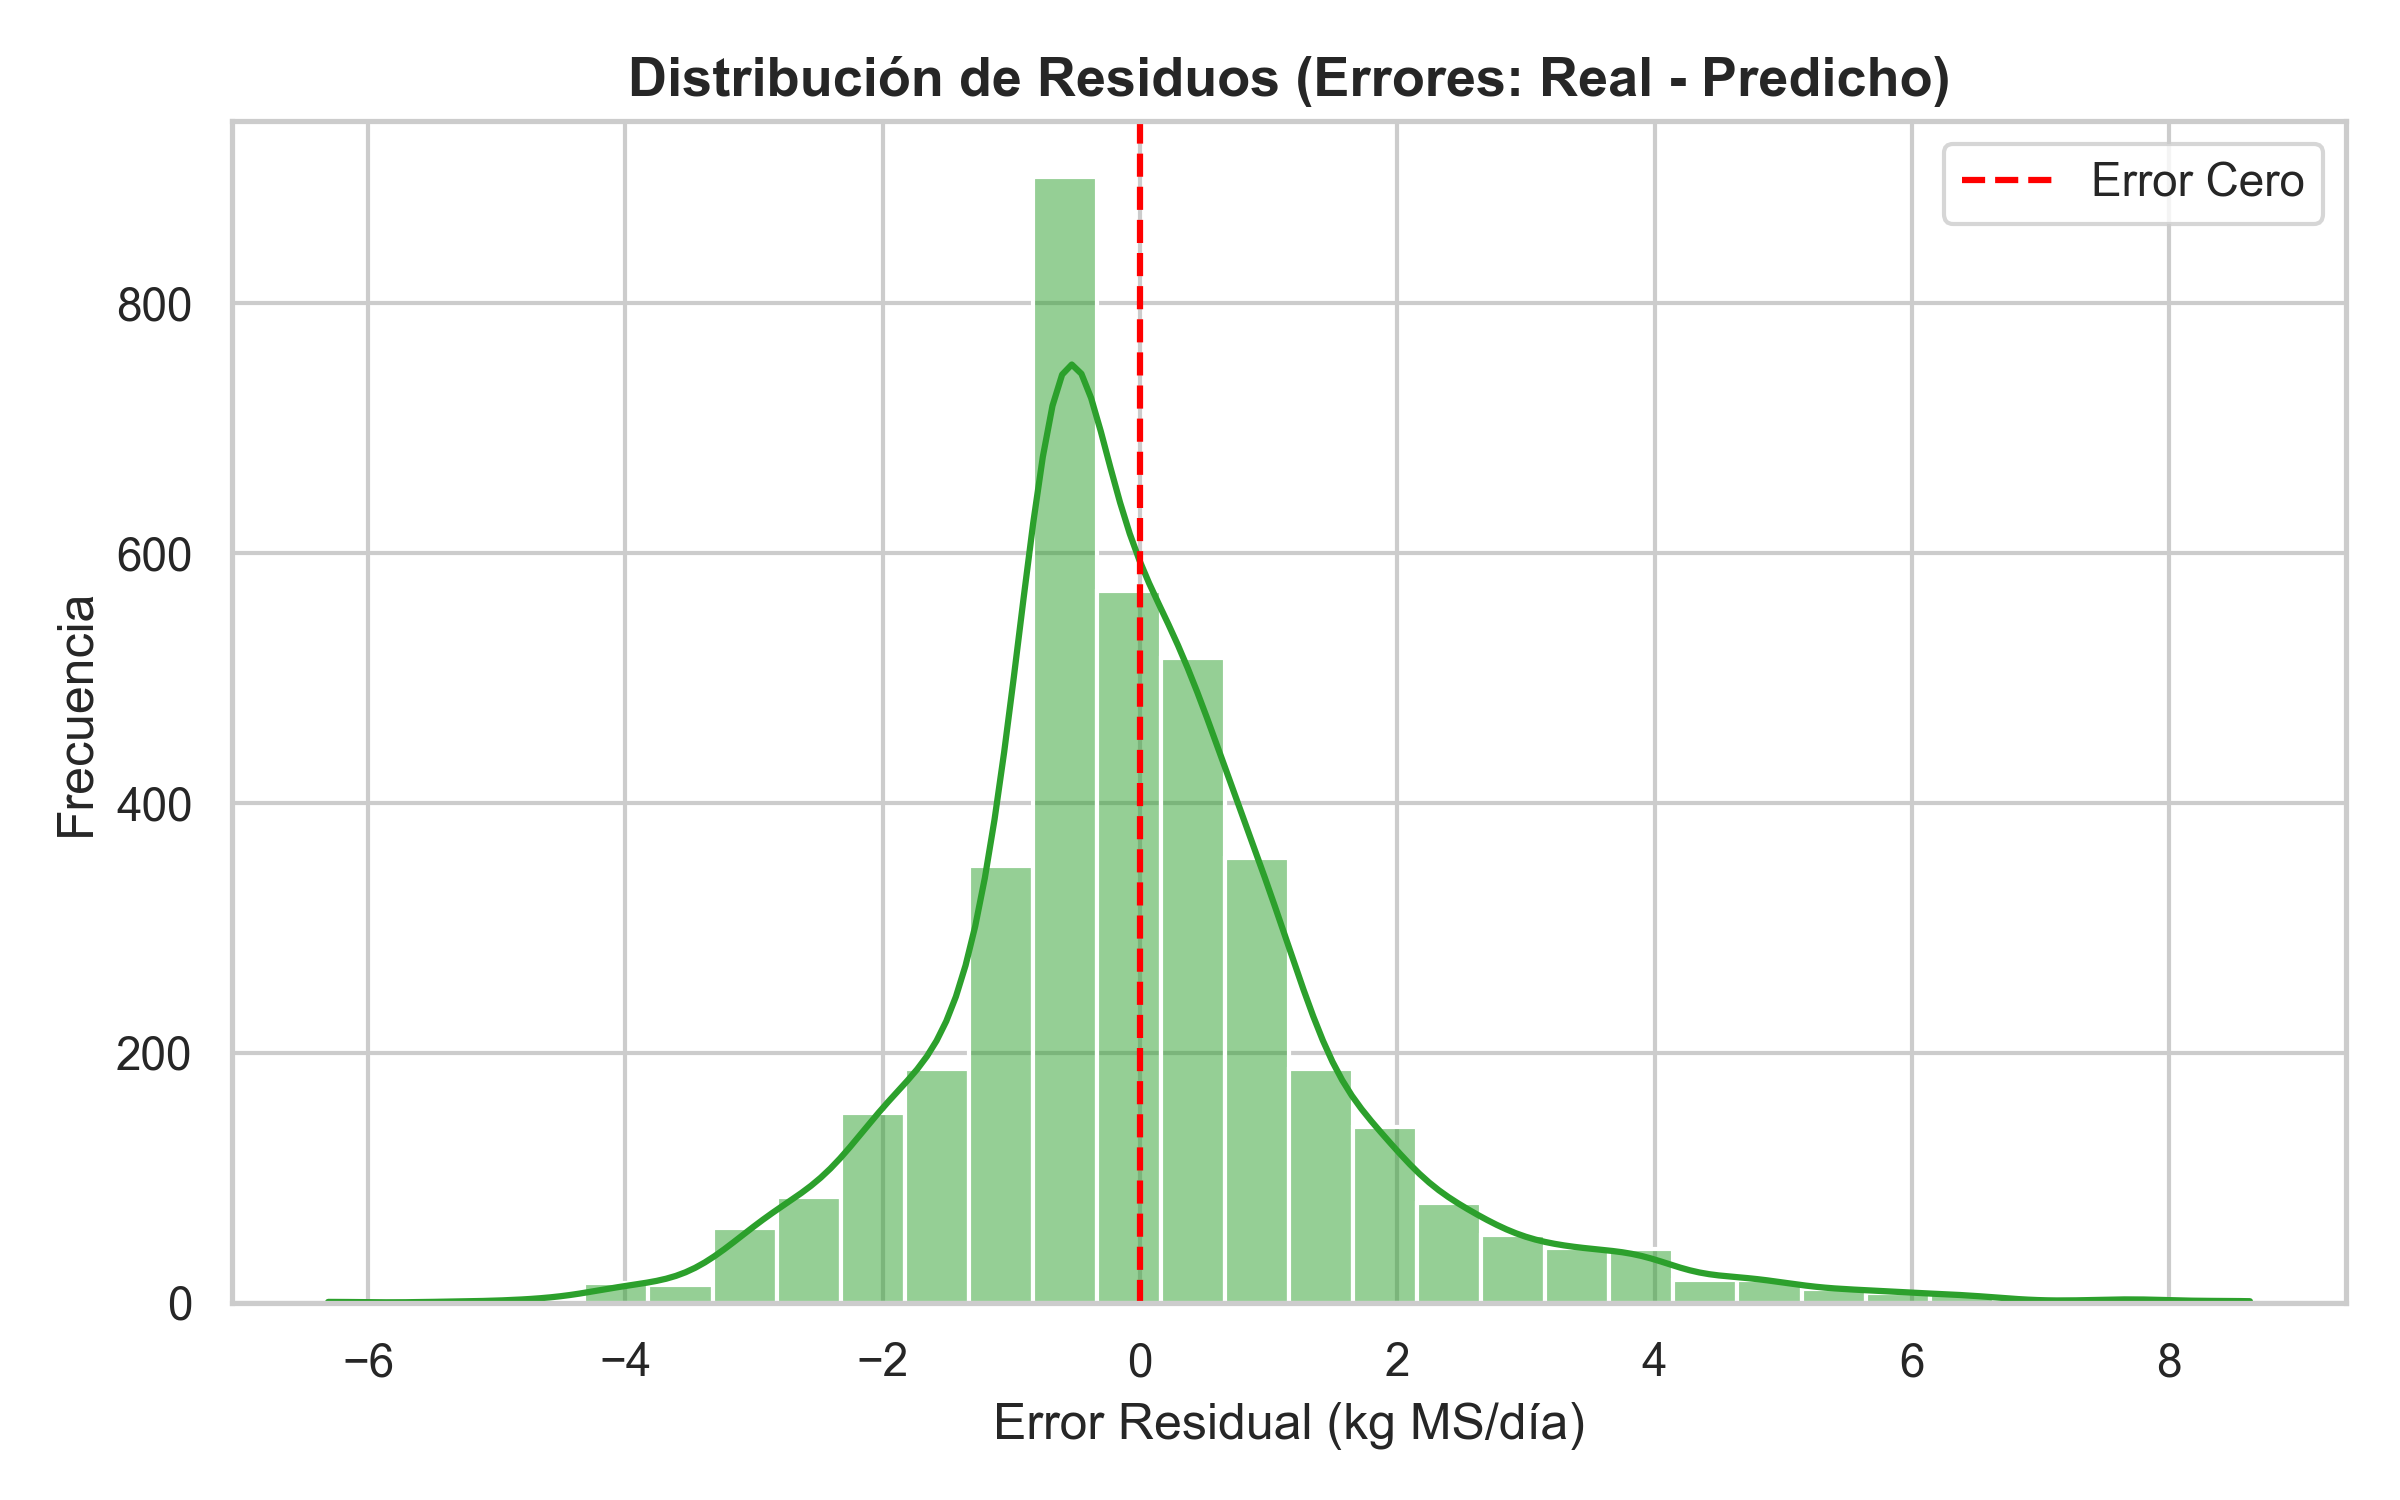
\includegraphics[width=0.9\textwidth]{figures/3_residuals_distribution.png}
\caption{Distribución de residuos. Un modelo ideal tendría errores centrados en cero, sin patrón y con dispersión reducida; el histograma por sí solo no comprueba normalidad ni homocedasticidad.}
\end{figure}

Los gráficos usan predicciones fuera de fold, decisión correcta para no mostrar artificialmente el ajuste sobre los mismos datos usados para entrenar. Faltan diagnósticos complementarios: residuos frente a predicción, QQ-plot, curvas de aprendizaje, error por hogar y periodo e intervalos de incertidumbre.

\section{Modelo final e interpretación}

El ganador formal es una \archivo{Pipeline} con preprocesador y Ridge. El bundle de 7.474 bytes contiene dos claves: \archivo{model} y \archivo{metadata}. El intercepto del Ridge ajustado es 4,6540485572.

\begin{table}[H]
\centering
\caption{Coeficientes del modelo final sobre variables transformadas.}
\small
\begin{tabular}{lr@{\qquad}lr}
\toprule
\textbf{Variable} & \textbf{Coef.} & \textbf{Variable} & \textbf{Coef.}\\
\midrule
Peso vivo estandarizado & 1,9508 & Estado B & 0,8753\\
Condición estandarizada & 0,2662 & Estado B/L & -0,1680\\
Indicador condición ausente & -0,0087 & DESCONOCIDO & -0,0922\\
Categoría Novillo & 0,3038 & Estado L & 0,9195\\
Categoría Ternero/Ternera & 0,2042 & Estado N & -0,8932\\
Categoría Toro & -0,4868 & Estado N/P & -0,0862\\
Categoría Vaca & 0,0043 & Estado P & -0,4730\\
Categoría Vaquilla & -0,0255 & Estado P/L & -0,0821\\
\bottomrule
\end{tabular}
\end{table}

El coeficiente 1,9508 de peso no significa 1,9508 kg de DMI por cada kilogramo de peso: corresponde al cambio asociado con una desviación estándar del peso después de escalar. Todos los niveles one-hot están incluidos; no existe una única categoría de referencia eliminada. Ridge resuelve la colinealidad mediante regularización, por lo que los coeficientes categóricos deben interpretarse en conjunto.

Tampoco son efectos causales. Un coeficiente puede recoger asociaciones con variables omitidas. Esto es especialmente importante para estados con una a cinco observaciones. Sin documentación sobre el significado de las siglas, no corresponde convertir esos números en conclusiones fisiológicas.

\begin{figure}[H]
\centering
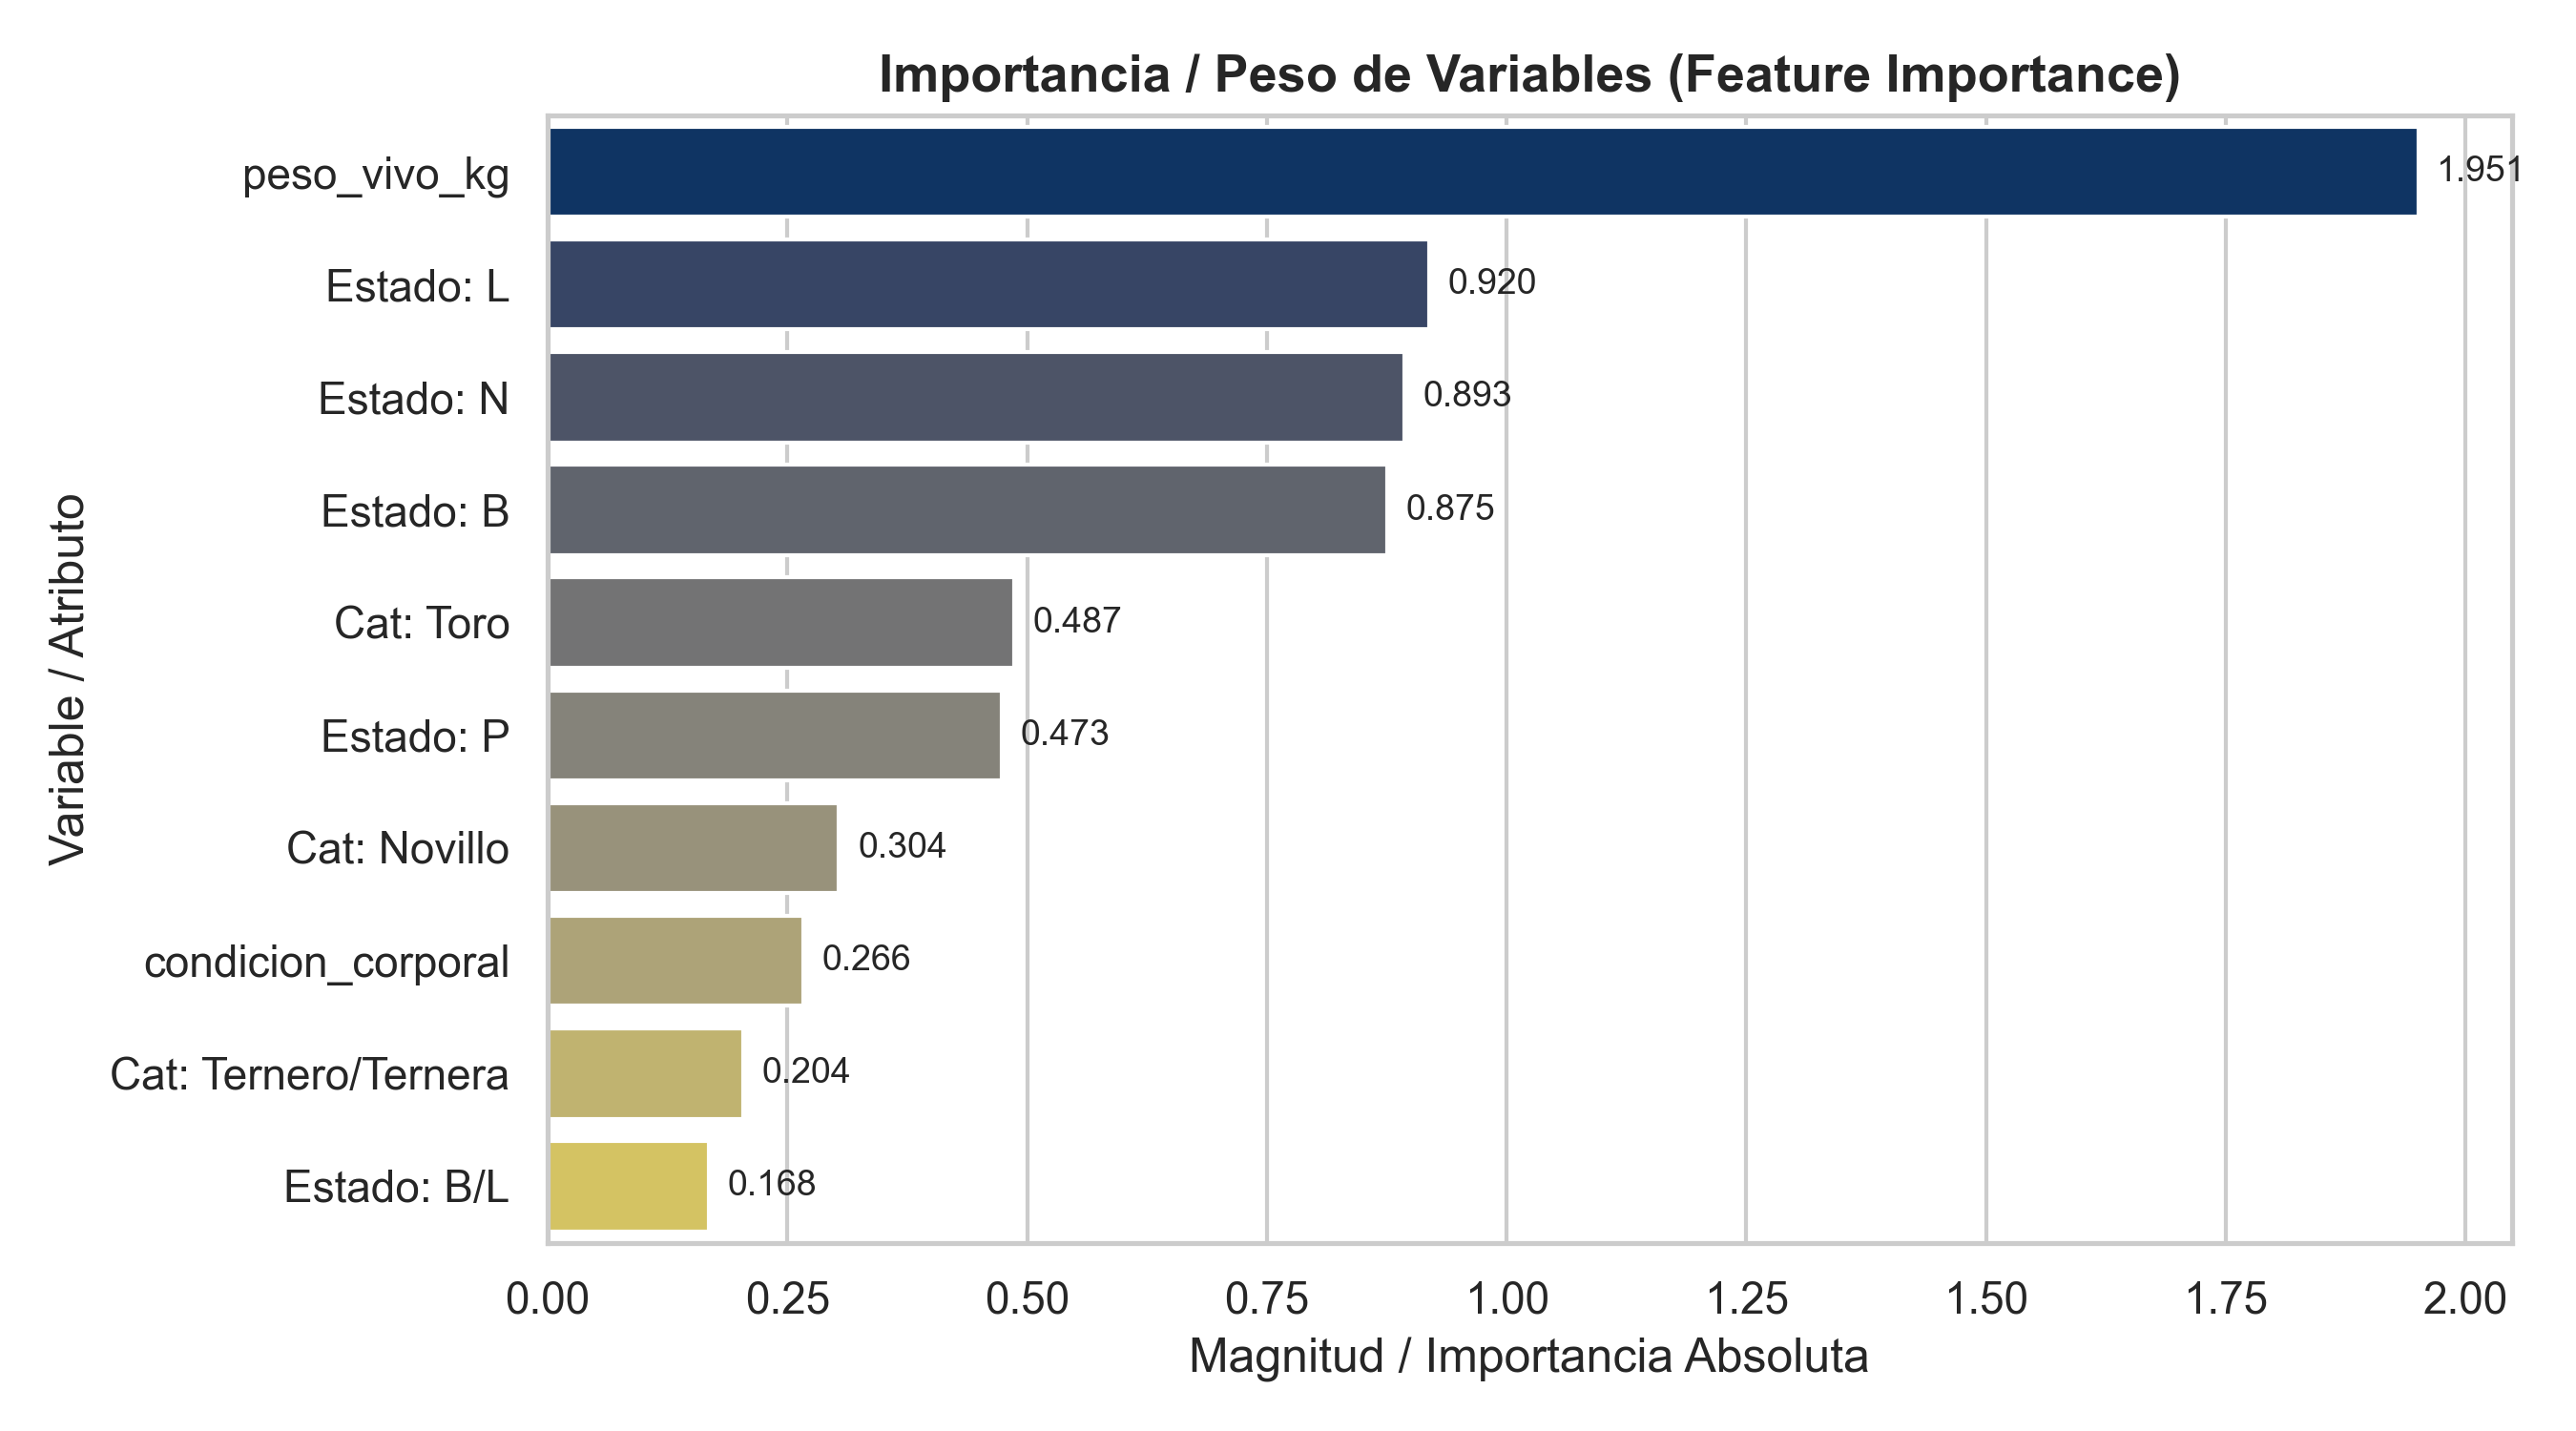
\includegraphics[width=0.9\textwidth]{figures/4_feature_importance.png}
\caption{Magnitud absoluta de coeficientes. En Ridge representa influencia en la escala transformada, no importancia causal ni necesariamente importancia por permutación.}
\end{figure}

\section{Inferencia y uso del modelo}

\subsection{Clase HerdPredictor}

Al construirse, \archivo{HerdPredictor} comprueba que exista el Joblib, carga el bundle y expone modelo y metadatos. Su método \archivo{predict(animals)} convierte una lista de diccionarios a DataFrame, prepara variables con el mismo contrato de entrenamiento, predice, aplica un piso de cero y devuelve por animal:
\begin{itemize}
  \item \archivo{animal_id};
  \item \archivo{dmi_kg_dia};
  \item \archivo{dmi_pct_peso_vivo}.
\end{itemize}

Los rangos de peso observados son 79,1--525,2 kg para Vaca; 54,6--412,8 para Vaquilla; 59,5--278,9 para Novillo; 97,0--595,5 para Toro; y 19,6--235,9 para Ternero/Ternera. Estar fuera del rango produce una advertencia, no un rechazo. La advertencia comunica extrapolación potencial: el rendimiento validado no cubre necesariamente esa entrada.

\subsection{Contrato JSON y ejemplo}

\begin{lstlisting}[language=Python]
{
  "animales": [
    {
      "animal_id": "A-001",
      "peso_vivo_kg": 420,
      "categoria_terrabovina": "Vaca",
      "condicion_corporal": 3.0,
      "estado_fisiologico_norm": "L"
    }
  ]
}
\end{lstlisting}

La prueba registrada contiene tres animales. A-001, vaca de 420 kg, obtiene 10,10 kg/día y 2,40\% PV; A-002, novillo de 400 kg, obtiene 8,53 kg/día y 2,13\% PV; A-003, vaca de 400 kg, obtiene 9,72 kg/día y 2,43\% PV. A-002 produce una advertencia porque 400 kg supera el máximo observado de 278,9 kg para novillos.

\subsection{Ejecución}

\begin{lstlisting}
python -m pip install -r requirements.txt
python -m src.etl.run_etl
python -m src.model.train
python testReal/ejecutar.py
\end{lstlisting}

El primer comando instala dependencias; el segundo ejecuta ETL; el tercero actualiza modelo, métricas y figuras; el cuarto lee \archivo{testReal/input.json} y sobrescribe \archivo{testReal/output.json}. Dado que actualmente no hay dataset raw, el ETL debe ejecutarse con precaución porque utiliza el procesado como fuente y destino.

\section{Calidad, limitaciones y amenazas a la validez}

\subsection{Inconsistencias documentales}

El README afirma 3.840 observaciones y tres modelos, pero el CSV y el reporte actuales contienen 3.833 filas y el código evalúa cuatro modelos. También menciona \archivo{pruebaModelo.py} y pruebas automáticas que están eliminadas del árbol actual. Otra explicación sostiene que se eliminaron siete atípicos desde 3.840 registros; esa reconstrucción puede ser histórica, pero \archivo{etl_summary.json} actual solo demuestra 3.833 entradas, cero eliminaciones y 3.833 salidas. El informe adopta los artefactos actuales y registra la discrepancia.

\subsection{Limitaciones metodológicas}

\begin{itemize}
  \item No existe conjunto de prueba externo ni validación con otra región.
  \item No hay validación temporal pese a los cuatro periodos.
  \item No hay búsqueda sistemática ni validación anidada de hiperparámetros.
  \item No se calculan intervalos de confianza, desviación entre folds ni pruebas pareadas.
  \item La selección considera únicamente MAE global, no estabilidad o equidad entre categorías.
  \item Algunos estados fisiológicos tienen entre una y cinco observaciones.
  \item No se proporcionan intervalos predictivos para cada animal.
  \item El agrupamiento por hogar es adecuado, pero las métricas siguen siendo internas al mismo dataset.
\end{itemize}

\subsection{Limitaciones de datos y validez externa}

Los datos provienen de Bomet, Kenia. No incluyen clima, calidad y disponibilidad del forraje, raza, edad exacta, producción láctea, composición de dieta, manejo ni condiciones productivas locales. El modelo aprende asociaciones de ese contexto; una métrica interna no garantiza precisión en Argentina. Además, 1.421 filas tienen \archivo{id_ambiguo=True}, pero ese indicador no se analiza ni filtra.

\subsection{Riesgos de ingeniería}

La inferencia no valida exhaustivamente identificadores, categorías, peso cero, condición corporal fuera de escala ni tamaño del lote. Una categoría desconocida puede interferir con la consulta de rangos. Joblib usa mecanismos de serialización equivalentes a Pickle y solo debe cargar archivos confiables. Faltan hashes, versionado de dataset, entorno exacto, CI y pruebas presentes. La normalización de estado está duplicada entre ETL y características, con riesgo de divergencia futura.

\section{Mejoras recomendadas}

\begin{enumerate}
  \item Conservar el CSV crudo inmutable, registrar su procedencia y generar versiones procesadas con hash.
  \item Corregir README y documentación para reflejar 3.833 filas, cuatro candidatos y comandos existentes.
  \item Restaurar y ampliar pruebas para ETL, esquema, entrenamiento, inferencia, gráficos y entradas inválidas.
  \item Declarar NumPy directamente y generar un archivo de dependencias bloqueadas.
  \item Evaluar validación temporal y un conjunto externo de establecimientos no representados.
  \item Comparar Ridge y CatBoost con repeticiones, intervalos y análisis pareado por hogar.
  \item Aplicar optimización de hiperparámetros dentro de validación anidada para evitar optimismo.
  \item Incorporar variables de dieta, clima, raza, edad, producción y manejo.
  \item Producir intervalos predictivos y criterios claros de abstención ante extrapolación.
  \item Validar entradas con un esquema formal y rechazar pesos imposibles o categorías desconocidas.
  \item Monitorear deriva de datos y error una vez disponibles observaciones reales posteriores.
\end{enumerate}

\section{Conclusiones}

El repositorio implementa un flujo completo y modular: valida y transforma datos, prepara características coherentes, compara modelos con separación por hogares, genera predicciones fuera de fold, persiste el ganador y ofrece inferencia por lotes. La exclusión de la variable derivada de DMI y el agrupamiento por finca son decisiones metodológicas importantes para reducir fuga de información.

Ridge obtiene MAE 1,1019 kg MS/día, RMSE 1,5354 y $R^2$ 0,6821, reduciendo aproximadamente 48,2\% el MAE del baseline. Su simplicidad, tamaño reducido e interpretabilidad favorecen su elección. No obstante, CatBoost alcanza MAE 1,1027: el empate práctico impide sostener que Ridge sea universalmente mejor. El rendimiento es menor en vacas, grupo de mayor consumo y variabilidad.

El proyecto demuestra viabilidad técnica para estimar DMI dentro de datos similares a los observados. No demuestra validez nutricional universal ni habilita uso directo en decisiones productivas argentinas. El paso siguiente más importante no es aumentar complejidad algorítmica, sino mejorar trazabilidad, recuperar datos crudos, obtener variables relevantes y validar externamente con datos locales.

\appendix
\section{Anexo: métricas por categoría de todos los modelos}

\small
\begin{longtable}{llrrr}
\toprule
\textbf{Modelo} & \textbf{Categoría} & \textbf{MAE} & \textbf{RMSE} & \textbf{$R^2$}\\
\midrule
\endhead
Baseline & Vaca & 2,3851 & 3,2324 & -0,4490\\
Baseline & Vaquilla & 1,5068 & 1,7483 & -0,3566\\
Baseline & Novillo & 1,3986 & 1,6071 & -1,3541\\
Baseline & Toro & 1,4650 & 1,9551 & -0,0129\\
Baseline & Ternero/Ternera & 2,6279 & 2,8295 & -5,7329\\
Ridge & Vaca & 1,5857 & 2,0608 & 0,4110\\
Ridge & Vaquilla & 0,7540 & 0,9449 & 0,6037\\
Ridge & Novillo & 0,6639 & 0,8028 & 0,4126\\
Ridge & Toro & 1,0204 & 1,3642 & 0,5068\\
Ridge & Ternero/Ternera & 0,5846 & 0,7018 & 0,5858\\
Random Forest & Vaca & 1,6903 & 2,2150 & 0,3196\\
Random Forest & Vaquilla & 0,8339 & 1,0338 & 0,5257\\
Random Forest & Novillo & 0,6563 & 0,8176 & 0,3907\\
Random Forest & Toro & 1,0924 & 1,4668 & 0,4299\\
Random Forest & Ternero/Ternera & 0,5469 & 0,6994 & 0,5886\\
CatBoost & Vaca & 1,5992 & 2,0923 & 0,3929\\
CatBoost & Vaquilla & 0,7732 & 0,9607 & 0,5904\\
CatBoost & Novillo & 0,6608 & 0,7952 & 0,4236\\
CatBoost & Toro & 1,0647 & 1,4755 & 0,4231\\
CatBoost & Ternero/Ternera & 0,5294 & 0,6604 & 0,6332\\
\bottomrule
\end{longtable}
\normalsize

\section{Anexo: archivos y salidas principales}

\begin{longtable}{p{6cm}p{9cm}}
\toprule
\textbf{Ruta} & \textbf{Contenido}\\
\midrule
\endhead
\archivo{src/config.py} & Rutas centrales del proyecto.\\
\archivo{src/etl/extract.py} & Lectura y contrato mínimo de siete columnas.\\
\archivo{src/etl/transform.py} & Limpieza, reglas, filtros y variable derivada.\\
\archivo{src/etl/load.py} & Escritura del CSV y resumen ETL.\\
\archivo{src/etl/run_etl.py} & Orquestación ejecutable del ETL.\\
\archivo{src/model/features.py} & Variables, categorías y preparación compartida.\\
\archivo{src/model/train.py} & Candidatos, validación, métricas, selección y persistencia.\\
\archivo{src/model/predictor.py} & Carga e inferencia por lotes.\\
\archivo{src/visualization/plots.py} & Generación de ocho gráficos a 300 DPI.\\
\archivo{models/dmi_model.joblib} & Pipeline Ridge final y metadatos.\\
\archivo{reports/model_metrics.json} & Métricas globales, por fold y categoría.\\
\archivo{reports/etl_summary.json} & Resultado de la última ejecución ETL.\\
\archivo{testReal/ejecutar.py} & Interfaz local mediante JSON.\\
\bottomrule
\end{longtable}

\section{Anexo: notas de lectura de los gráficos}

La comparación de modelos responde qué candidato obtiene menor error agregado. El gráfico real-predicho permite identificar dispersión y posibles sesgos de escala. Los residuos muestran forma y asimetría del error, pero deben complementarse con residuos frente a predicción. La magnitud de coeficientes sirve para explicar Ridge en la escala transformada. El MAE por categoría revela heterogeneidad. Los gráficos de peso y boxplots describen el dataset y no el desempeño causal. La matriz de correlación resume asociación lineal y puede ocultar interacciones o no linealidad.

Todas las figuras incluidas fueron producidas por \archivo{src/visualization/plots.py} a partir del dataset y, cuando corresponde, de predicciones out-of-fold del modelo ganador.

\end{document}
